%% For double-blind review submission
\documentclass[acmlarge,anonymous]{acmart}\settopmatter{printfolios=true}
%% For single-blind review submission
%\documentclass[acmlarge,review]{acmart}\settopmatter{printfolios=true}
%% For final camera-ready submission
%\documentclass[acmlarge]{acmart}\settopmatter{}

%% Note: Authors migrating a paper from PACMPL format to traditional
%% SIGPLAN proceedings format should change 'acmlarge' to
%% 'sigplan,10pt'.


%% Some recommended packages.
\usepackage{wrapfig}
\usepackage{mathtools}
\usepackage{mathpartir}
\usepackage{fullpage}
\usepackage{ifpdf}
\usepackage{graphicx}
%\usepackage[usenames,dvipsnames]{color}
\usepackage{subcaption}
\usepackage{stmaryrd}
%\usepackage[numbers]{natbib}
\usepackage{amsthm}
\usepackage{listings}          % format code
\usepackage{xspace}

% Math mode
%-----------
\newenvironment{nop}{}{}
\newenvironment{smathpar}{
\begin{nop}\small\begin{mathpar}}{
\end{mathpar}\end{nop}\ignorespacesafterend}

% Name
%-----
\newcommand{\name}{{\sc vml}\xspace}
\newcommand{\nameMonad}{{\sc vst}\xspace}

% Formatting
%---------
\newcommand{\C}[1]{\code{#1}}
\newcommand{\tuplee}[1]{\langle #1 \rangle}
\newcommand*{\rom}[1]{\expandafter\romannumeral #1}

% Formatting commands
% -------------------
\newcommand{\code}[1]{\,{\tt #1}\,}
\newcommand{\spc}[0]{\quad}
\newcommand{\ALT}{~\mid~}
\newcommand{\rel}[1]{{R}_{\mathit{#1}}}
\newcommand{\conj}{~\wedge~}
\newcommand{\disj}{~\vee~}
\newcommand{\rulelabel}[1]{\textrm{\sc {#1}}}
\newcommand{\ilrulelabel}[1]{{\sc #1}}
\newcommand{\RULE}[2]{\frac{\begin{array}{c}#1\end{array}}
                           {\begin{array}{c}#2\end{array}}}
\newcommand{\denot}[1]{\llbracket #1 \rrbracket}
\newcommand{\bind}{>\!\!>\!\!=}
\ifx\coloneqq\undefined
  \newcommand{\coloneqq}{::=}
\else
  \renewcommand{\coloneqq}{::=}
\fi
\newcommand{\stepsto}{\longrightarrow}
\newcommand{\return}[1]{\C{return}\;#1}
\newcommand{\run}[2]{\C{run}\;#1\;#2}
\newcommand{\fork}[1]{\C{fork}\;#1}
\newcommand{\push}[1]{\C{push}\;#1}
\newcommand{\pull}{\C{pull}}
\newcommand{\semsucceq}{\succeq_{\circ}}
\newcommand{\sempreceq}{\preceq_{\circ}}
\newcommand{\under}[2]{#1\,\vdash\,#2}
\newcommand{\mbleto}{\rightsquigarrow_m}
\newcommand{\drawsome}{{\sf Canvas}\xspace}
\newcommand{\buylist}{{\sf ToBuy}\xspace}
\newcommand{\lang}{\lambda_b}
\newcommand{\length}[1]{\left|#1\right|}
\newcommand{\GK}[1]{\textcolor{red}{GK: #1}}

% New colors
%------------
\definecolor{Bittersweet}{rgb}{1.0, 0.44, 0.37}
\definecolor{MidnightBlue}{rgb}{0.0, 0.2, 0.4}

% Listings Code
%---------------
\newcommand{\lstml}{
\lstset{ %
language=ML, % choose the language of the code
basicstyle=\footnotesize\ttfamily,       % the size of the fonts that are used for the code
keywordstyle=\color{Bittersweet},
% numbers=left,                   % where to put the line-numbers
numberstyle=\tiny,      % the size of the fonts that are used for the line-numbers
stepnumber=1,                   % the step between two line-numbers. If it is 1 each line will be numbered
numbersep=5pt,                  % how far the line-numbers are from the code
showspaces=false,               % show spaces adding particular underscores
showstringspaces=false,         % underline spaces within strings
showtabs=false,                 % show tabs within strings adding particular underscores
% frame=single,                   % adds a frame around the code
tabsize=2,                      % sets default tabsize to 2 spaces
captionpos=b,                   % sets the caption-position to bottom
breaklines=true,                % sets automatic line breaking
breakatwhitespace=false,        % sets if automatic breaks should only happen at whitespace
commentstyle=\itshape\color{MidnightBlue},
%escapeinside={\%*}{*)},         % if you want to add a comment within your code
morekeywords={module, match, when, @@deriving, not, : , /\\}
}}
\lstnewenvironment{ocaml}
    { % \centering
			\lstml
      \lstset{}%
      \csname lst@setfirstlabel\endcsname}
    { %\centering
      \csname lst@savefirstlabel\endcsname}



\makeatletter\if@ACM@journal\makeatother
%% Journal information (used by PACMPL format)
%% Supplied to authors by publisher for camera-ready submission
\acmJournal{PACMPL}
\acmVolume{1}
\acmNumber{1}
\acmArticle{1}
\acmYear{2017}
\acmMonth{1}
\acmDOI{10.1145/nnnnnnn.nnnnnnn}
\startPage{1}
\else\makeatother
%% Conference information (used by SIGPLAN proceedings format)
%% Supplied to authors by publisher for camera-ready submission
\acmConference[PL'17]{ACM SIGPLAN Conference on Programming Languages}{January 01--03, 2017}{New York, NY, USA}
\acmYear{2017}
\acmISBN{978-x-xxxx-xxxx-x/YY/MM}
\acmDOI{10.1145/nnnnnnn.nnnnnnn}
\startPage{1}
\fi


%% Copyright information
%% Supplied to authors (based on authors' rights management selection;
%% see authors.acm.org) by publisher for camera-ready submission
\setcopyright{none}             %% For review submission
%\setcopyright{acmcopyright}
%\setcopyright{acmlicensed}
%\setcopyright{rightsretained}
%\copyrightyear{2017}           %% If different from \acmYear


%% Bibliography style
\bibliographystyle{ACM-Reference-Format}
%% Citation style
%% Note: author/year citations are required for papers published as an
%% issue of PACMPL.
\citestyle{acmauthoryear}   %% For author/year citations

\newcommand{\KC}[1]{{\textcolor{red}{{KC: #1}}}}

\begin{document}

%% Title information
\title[]{Mergeable Types}         %% [Short Title] is optional;
                                        %% when present, will be used in
                                        %% header instead of Full Title.
%\titlenote{with title note}             %% \titlenote is optional;
                                        %% can be repeated if necessary;
                                        %% contents suppressed with 'anonymous'
%\subtitle{Subtitle}                     %% \subtitle is optional
%\subtitlenote{with subtitle note}       %% \subtitlenote is optional;
                                        %% can be repeated if necessary;
                                        %% contents suppressed with 'anonymous'


%% Author information
%% Contents and number of authors suppressed with 'anonymous'.
%% Each author should be introduced by \author, followed by
%% \authornote (optional), \orcid (optional), \affiliation, and
%% \email.
%% An author may have multiple affiliations and/or emails; repeat the
%% appropriate command.
%% Many elements are not rendered, but should be provided for metadata
%% extraction tools.

%% Author with single affiliation.
\author{First1 Last1}
\authornote{with author1 note}          %% \authornote is optional;
                                        %% can be repeated if necessary
\orcid{nnnn-nnnn-nnnn-nnnn}             %% \orcid is optional
\affiliation{
  \position{Position1}
  \department{Department1}              %% \department is recommended
  \institution{Institution1}            %% \institution is required
  \streetaddress{Street1 Address1}
  \city{City1}
  \state{State1}
  \postcode{Post-Code1}
  \country{Country1}
}
\email{first1.last1@inst1.edu}          %% \email is recommended

%% Author with two affiliations and emails.
\author{First2 Last2}
\authornote{with author2 note}          %% \authornote is optional;
                                        %% can be repeated if necessary
\orcid{nnnn-nnnn-nnnn-nnnn}             %% \orcid is optional
\affiliation{
  \position{Position2a}
  \department{Department2a}             %% \department is recommended
  \institution{Institution2a}           %% \institution is required
  \streetaddress{Street2a Address2a}
  \city{City2a}
  \state{State2a}
  \postcode{Post-Code2a}
  \country{Country2a}
}
\email{first2.last2@inst2a.com}         %% \email is recommended
\affiliation{
  \position{Position2b}
  \department{Department2b}             %% \department is recommended
  \institution{Institution2b}           %% \institution is required
  \streetaddress{Street3b Address2b}
  \city{City2b}
  \state{State2b}
  \postcode{Post-Code2b}
  \country{Country2b}
}
\email{first2.last2@inst2b.org}         %% \email is recommended


%% Paper note
%% The \thanks command may be used to create a "paper note" ---
%% similar to a title note or an author note, but not explicitly
%% associated with a particular element.  It will appear immediately
%% above the permission/copyright statement.
%\thanks{with paper note}                %% \thanks is optional
                                        %% can be repeated if necesary
                                        %% contents suppressed with 'anonymous'


%% Abstract
%% Note: \begin{abstract}...\end{abstract} environment must come
%% before \maketitle command
\begin{abstract}
  Distributed applications often replicate data to improve
  availability and fault tolerance.  But, the use of replication leads
  to a significantly more complex and onerous programming model.  To
  ensure a sensible measure of consistency among different replicas of
  an object, applications are typically structured so that the
  operations applied to a replicated object on one node are
  subsequently communicated to other nodes where they can be
  re-applied locally.  Oftentimes, the degree of restructuring and
  care necessary to transform a sequential or shared-memory concurrent
  application to a meaningful (replicated) distributed one can be
  substantial.

  In this paper, we present a new interpretation of replicated types
  that overcome these concerns.  Our declarative programming model
  called \name\ treats replication as a compositional form of
  versioning, in which consistency is enforced through
  programmer-supplied \emph{merge} functions.  Distributed state is
  now viewed in terms of a tree of immutable object versions, with
  merge actions used explicitly by the application or implicitly by
  the underlying runtime system to periodically reconcile local
  versions to yield a consistent global state.  Our model frees the
  programmer from having to think of low-level operational notions
  related to distribution and replication, and therefore does not
  entail any restructuring of application logic to enable distributed
  programming.

  We show how any ML datatype can be enriched to support mergeability,
  formalize a concurrency semantics based on such types, and describe
  an instantiation of OCaml equipped with these features.  Our
  implementation is integrated with a content-addressable distributed
  storage layer that allows any OCaml program to be easily transformed
  into a composable, efficient, and highly-available distributed
  application.
\end{abstract}


%% 2012 ACM Computing Classification System (CSS) concepts
%% Generate at 'http://dl.acm.org/ccs/ccs.cfm'.
\begin{CCSXML}
<ccs2012>
<concept>
<concept_id>10011007.10011006.10011008.10011009.10010177</concept_id>
<concept_desc>Software and its engineering~Distributed programming languages</concept_desc>
<concept_significance>500</concept_significance>
</concept>
<concept>
<concept_id>10011007.10011006.10011008.10011024.10011028</concept_id>
<concept_desc>Software and its engineering~Data types and structures</concept_desc>
<concept_significance>500</concept_significance>
</concept>
<concept>
<concept_id>10011007.10011006.10011039.10011311</concept_id>
<concept_desc>Software and its engineering~Semantics</concept_desc>
<concept_significance>300</concept_significance>
</concept>
<concept>
<concept_id>10003752.10010124.10010125.10010130</concept_id>
<concept_desc>Theory of computation~Type structures</concept_desc>
<concept_significance>300</concept_significance>
</concept>
</ccs2012>
\end{CCSXML}

\ccsdesc[500]{Software and its engineering~Distributed programming languages}
\ccsdesc[500]{Software and its engineering~Data types and structures}
\ccsdesc[300]{Software and its engineering~Semantics}
\ccsdesc[300]{Theory of computation~Type structures}

%% End of generated code


%% Keywords
%% comma separated list
\keywords{Replicated Datatypes, Eventual Consistency, Availability, CRDTs, Versions, ML}  %% \keywords is optional


%% \maketitle
%% Note: \maketitle command must come after title commands, author
%% commands, abstract environment, Computing Classification System
%% environment and commands, and keywords command.
\maketitle


\section{Introduction}
\label{sec:intro}

Real-world distributed programs are challenging to write and maintain
because they often conflate two distinct mechanisms.  The first
concerns the expression of application logic - how do we define
computations that are robust in the presence of distributed
communication among concurrently executing threads of control?  The
second deals with system concerns - how do we express notions of
visibility, replication, and consistency when the nodes participating
in such computations may be geographically distributed and the
networks that connect them unreliable?  To simplify reasoning in such
complicated environments, programming models often make strong
assumptions on the guarantees provided by an implementation (such as
serializability~\cite{Serializability} or strong
consistency~\cite{CDE+12,DNN+15}) that may inadvertently mask,
restrict, or ignore important albeit unpleasant realities (e.g.,
network partitions~\cite{Brewer2000,Gilbert2002}). When unwarranted
assumptions are made, program behavior is often difficult to predict
and verify.  On the other hand, when these features are explicitly
exposed to the programmer, e.g., by requiring that applications be
written in terms of specialized distributed data
structures~\cite{Burckhardt2014,BFL+12,SPB+11} or control
primitives~\cite{Calm}, simplicity, composability, and
ease-of-reasoning can suffer.

To illustrate how these kinds of problems manifest in practice,
consider how we might write a simple counter library (see
Fig.~\ref{fig:counter-adt}).  A \C{Counter} supports two (update)
operations - \C{add} and \C{mult} - that lets a non-negative integer
value be added or multiplied to the counter, resp.  Observe that the
library is written in an idiomatic functional style, with no special
reasoning principles needed to realize desired functionality.  As long
as applications use the library on a single machine, this
implementation behaves as expected.  However, if the library is used
in the context of a more sophisticated application, say one whose
computation is distributed among a collection of machines, its
behavior can become significantly harder to understand.  In
particular, a distributed implementation might wish to
\emph{replicate} the counter state on each node to improve response
time or fault tolerance.  Unfortunately, adding replication doesn't
come for free.  Attempting to update every replicated copy atomically
is problematic in the absence of sophisticated transaction support,
which impose significant performance penalties.  But, without such
heavyweight mechanisms, applying an \C{Add} operation on one node may
not be instanteously witnessed on another, which may be in the process of
simultaneously attempting to perform its own \C{Add} or \C{Mult}
action.  While synchronizing the activities of all nodes to ensure at
most one such operation is performed at a time is impractical,
designating a single node to hold the counter state eschewing
replication altogether (as in a client-server
configuration~\cite{Armstrong}), is also an undesirable solution,
given the sensitivity of such architectures to network partitions and server failures, and
the negative performance impact it incurs in geo-distributed
environments~\cite{Walter}.  Removig coordination altogether by simply
replicating counter state without having any supporting consistency
protocol is an equally infeasible approach.

A method often adopted to address these concerns is to re-define a
datatype's operations to return \emph{effects} instead of
values~\cite{SPB+11,Burckhardt2014}.  An \emph{effect} is a tag that
identifies the operation to be applied uniformly at all replicas to
incorporate the effects of the original
operation. Fig.~\ref{fig:counter-rdt} shows the \C{Counter} library
with operations re-defined to returns effects.  Observe that the
\C{Counter.add x v} operation now returns an \C{Add x} effect, which,
when applied at a replica (see \C{apply} in the figure), adds \C{x} to
the local counter value.  Note, however, that \C{add} and \C{mult} are
not commutative operations - assuming two replicas have the same
initial counter value of 0, applying the effect of adding 3 and then
multiplying 5 on one replica yields 15, while applying the effect of
first multiplying 5 and then adding 3 yields 3 on the other.  Such
scenarios are possible in a distributed system because there are no
coherence guarantees on the order in which effects are received by
different nodes.  Thus, implementations must be carefully written to
take the lack of commutativity into account when defining how effects
are applied at a replica; in the figure, multiplication is expressed
in terms of addition to avoid the kind of undesirable behavior
described above.

In this implementation, all replicas will eventually contain the same
counter value, assuming updates to the counter eventually quiesces.
While transmitting effects provide a low-level operational basis for
handling replicated state, the \emph{ad hoc} nature of the solution
confounds desirable high-level reasoning principles.  Indeed, the
semantic gap between the two versions of the counter, one cognizant of
replication and the other not, breaks backward compatibility with the
original state-based implementation.  Just as significantly, its
non-trivial construction must be developed in different guises for
every distributed data structure used by the application.
\begin{figure}
\begin{subfigure}[b]{0.4\textwidth}
  \begin{ocaml}
    module Counter: sig
      type t
      val add: int -> t -> t
      val mult: int -> t -> t
      val read: t -> int
    end = struct
      type t = int
      let add x v = v + (abs x)
      let mult x v = v * (abs x)
      let read v = v
    end
  \end{ocaml}
\caption{\C{Counter} library in OCaml}
\label{fig:counter-adt}
\end{subfigure}
\begin{subfigure}[b]{0.56\textwidth}
  \begin{ocaml}
    module Counter: sig
      type t
      type eff
      val add: int -> t-> eff
      val mult: int -> t -> eff
      val apply: eff -> t -> t
      val read: t -> int
    end = struct
      type t = int
      type eff = Add of int
      let add x v = Add (abs x)
      let mult x v = Add (v * (abs x - 1))
      let apply (Add x) v = x + v
      let read v = v
    end
  \end{ocaml}
\caption{\C{Counter} library re-engineered for effect-based replication}
\label{fig:counter-rdt}
\end{subfigure}
\end{figure}
The lack of composability is yet another important downside of this
approach.  Consider an application that uses two replicated counters,
$c_1$ and $c_2$, bound by the invariant $c_2 \ge c_1$, duly enforced
by the application when updating $c_2$ or $c_1$.  An execution may
nonetheless witness anamolous states that violate the invariant
because updates to $c_1$ and $c_2$ may be applied independently in any
order on any replica.  For example, if a replica increments both
counters, a \C{read} operation performed at another replica may
\begin{wrapfigure}{l}{.5\textwidth}
  \begin{center}
    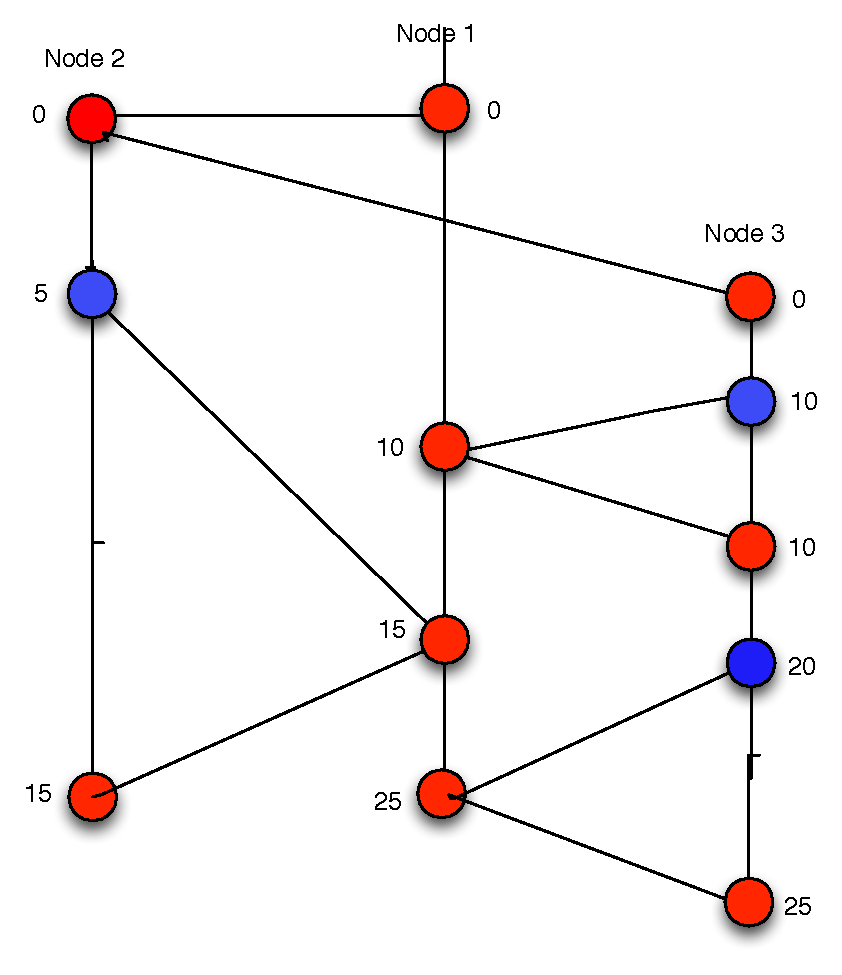
\includegraphics[scale=0.4]{Figures/dali-counter}
  \end{center}
  \caption{\small A replicated counter can be expressed as a sequence
    of versions managed by logically-distributed concurrently
    executing threads.  Local versions produced by these threads
    periodically merge their state with one another.  In the figure,
    when the local version of Node 3, labeled 20, merges with the
    local version of Node 1, whose counter state is 15 at the time, a
    new counter value is produced.  This value takes into account the
    previous merged state (10) from which the two versions were
    derived to yield a new merged state of 25.  There is no other form
    of synchronization or coordination among versions except through
    merging.  In the figure, red circles represent counter state
    produced through merging, and blue circles represent state
    produced by applying counter operations on a node-local version.
  }
\vspace*{-.85in}
\end{wrapfigure}
witness the increment to $c_1$, but not $c_2$, thus violating the
invariant. The intention to atomically apply both effects cannot be
captured in the absence of external mechanisms to compose effects
(such as effect-based transactions~\cite{pldi15}).  Rather than
viewing a distributed computation in terms of \C{Add} effects produced
by operations, can we formulate a more declarative interpretation,
directly in terms of the counter value maintained by each node.  In
doing so, we observe that each replica essentially operates over its
own version of a counter.  Local operations on a replicated object can
be thought of as yielding new versions, thus producing a version tree,
with one branch for each replica.  Thus, every branch represents
different (immutable) versions maintained by different nodes, with the
state produced by the computation performed over a counter on a node
recorded along the node's local branch for the counter.  Now, to
generate a globally consistent view of a counter, we only need to
define a merge operation that explains how to combine two local
versions to produce a new version that reflects both their states.

Framing replication as merging leads to a counter implementation that
bears strong similarity to the original sequential one:
  \begin{ocaml}
    module Replicated_Counter = struct
      include Counter
      let merge lca v1 v2 =
         lca + (v1 - lca) + (v2 - lca)
    end
  \end{ocaml}
The role of \C{lca} (least common ancestor) here captures salient
history - the state resulting from the merge of two versions derived
from the same ancestor state should not unwittingly duplicate the
contributions of the ancestor.  This interpretation of a replicated
datatype is thus given in terms of the evolution of a program state
impicitly associated with the different nodes that comprise a
distributed application with merge operations serving to communicate
and reconcile different local states.

In this paper, we develop a programming model that realizes a monadic
version control system centered around data, rather than file,
coherence.  The \name monad lets programmers write and compose
concurrent computations around multiple (implicit) versions of a
mergeable datatype, an ordinary ML datatype additionally equipped with
a \emph{merge} function responsible for deriving a consistent global
state from a collection of local versions of that state.  A
computation progresses by forking (i.e., replicating) new versions of
existing versions on geo-distributed nodes, allowing
synchronization-free local computation to proceed on those nodes,
creating new versions along an existing \emph{branch} that represents
updated local instances, and by merging branches to realize global
consistency.

Our model allows ML programmers to get the benefits of achieving
highly available (low-latency) distributed computation, while
continuing to enjoy the comforts of high-level reasoning and the
familiarity of using standard libraries already provided by the
language.  Notably, while \name's programming model makes no explicit
reference to any specific operational manifestation of a distributed
system (e.g., programmers do not need to explicitly manage replicas),
we demonstrate that it can be nonetheless efficiently realized on
existing geo-replicated distributed systems.

Our contributions are summarized below:

\begin{itemize}
    \item We formally introduce the concept of a \emph{mergeable}
      datatype to admit high-level declarative reasoning about
      distributed computation and replicated state in ML programs.

    \item We describe \name programming model that brings to bear the
      power and flexibility of a version control system to the
      administration of replicated data. \name hides the complexity of
      version control behind a monad, and exposes its functionality
      via a simple API that lets programmers define and compose
      distributed ML computations around such data.  Issues related to
      replication only manifest implicitly in the definition of a
      merge operation that defines coherence among different instances
      of replicated state.

    \item We present a formalization of the \name programming model,
      and establish the comditions under which eventual convergence of
      concurrent version state can be guaranteed.

    \item We describe an implementation of the \name library that
      transparently adds persistence and replication features to a
      mergeable type, and which sits atop the Irmin persistent
      store~\cite{irmin}, a content-addressable storage library for
      OCaml. We also present case studies and experimental results
      that justify the practical utility of our approach.
\end{itemize}

The remainder of the paper is organized as follows.  We present the
\name\ programming model informally in the next section.
Sec.~\ref{sec:mergeable_types} develops a series of examples that
illustrate how merge operations can be defined and used.
Sec.~\ref{sec:formalization} defines an operational semantics, and
formalizes our intution of a mergeable type in terms of morphisms over
datatype operations.  We also present soundness (consistency) and
progress guarantees enjoyed by the
semantics. Sec.~\ref{sec:system-model} considers an instantiation of
the model suitable for distributed environments with network
partitions and failures.  Implementation details describing how we
incorporate mergeable types into OCaml are presented in
Sec.~\ref{sec:impl}.  Experimental results and benchmarks are given
in Sec.~\ref{sec:evaluation}.



, along with
a series of examples illustrating how merge operations can be defined
and used.  Sec.~\ref{sec:


%% Persistence adds yet another dimension to the problem. Functional data
%% structures are often large in-memory linked structures that admit
%% functional updates by creating newer versions that share most of their
%% structure with previous versions. Sharing is the key to efficiency,
%% without which every functional update takes time that is at least
%% linear in the size of the data structure. Unfortunately, the
%% straightforward way to persist a data structure on disk in a
%% machine-agnostic format (e.g., JSON) requires serialization, which is
%% linear in the size of the data structure. An alternative is to
%% maintain a separate on-disk copy of the data and administer it via a
%% database system. The downside is that the programmer is now required
%% to reason in terms of a lower-level abstraction (e.g., a relational
%% data model) in order to maintain coherence between in-memory and
%% on-disk representations. Safety guarantees over the in-memory data do
%% not carry over to the disk, which introduces additional complications
%% and the possibility of new bugs. Thus, adding persistence to
%% applications while preserving high-level safety gurantees offered by
%% the language abstraction is a non-trivial problem.



%% However, as we shall see,
%% unconstrained branching may yield a branching structure that becomes
%% unmergeable, thus leading to \emph{stuck} states. An important
%% property of the \name library is that it guarantees progress even in
%% the presence of arbitrary merges provided the merge operation is
%% commutative with respect to its version state arguments.  Furthermore,
%% \name profitably exploits provenance information available via
%% branches to make application resilient to network partitions.
%% In this paper, we define a semantics of mergeable datatypes that lets
%% any OCaml program be seamlessly deployed in a distributed environment
%% with implicit support for replicated and decentralized operation.  The
%% underlying foundation for merge actions has a natural category
%% theoretic interpretation that enables us to construct useful mergeable
%% variants for \emph{any} OCaml type whose states are commutative wtih
%% respect to the merge operation defie


\section{Programming Model}

\begin{figure}
\begin{center}
  \begin{ocaml}
  module type CANVAS = sig
    type pixel = {r:char; g:char; b:char}
    type tree = 
      | N of pixel
      | B of {tl: tree; tr: tree; bl: tree; br: tree} 
    type t = {max_x:int; max_y:int; canvas:tree} 
    type loc = {x:int; y:int}
  
    val new_canvas: int -> int -> t
    val set_px: t -> loc -> pixel -> t
    val get_px: t -> loc -> pixel
    val merge: (* lca *)t -> (* v1 *)t -> (* v2 *)t -> t
  end
  \end{ocaml}
\end{center}
\caption{\drawsome: a sample \name application}
\label{fig:canvas-sig}
\end{figure}

In this section, we describe the \name programming model through the
example of a collaborative drawing application we call \drawsome.

Fig.~\ref{fig:canvas-sig} shows the signature of the \drawsome
application. \drawsome represents a free-hand drawing canvas in terms
of a tree of quadrants.  Each quadrant is simply a leaf node
containing a single pixel (\C{r},\C{g}, or \C{b}) or a tree, if the
quadrant contains multiple pixels of different colors. Quadrants are
expanded into a tree structures as and when pixels are colored.  The
representation is thus optimized for sparse canvases, such as
whiteboards. The application supports three simple operations:
creating a new canvas, setting the pixel at a specified coordinate,
and returning the pixel at a given coordinate. The \C{merge} function
and \C{deriving versioned} directive are explained below.

\begin{figure}
\centering
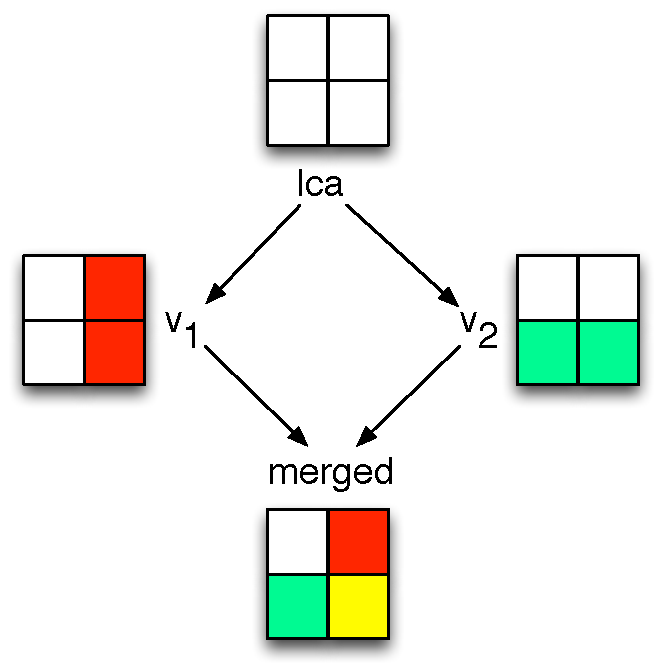
\includegraphics[scale=0.5]{Figures/canvas-merging}

\caption{Merging concurrent versions (\C{v1} and \C{v2} ) of a drawing
canvas. \C{lca} is their common ancestor.}
\label{fig:canvas-merging}
\end{figure}

\drawsome lets multiple users collaborate on a canvas that is
conceptually shared among them. Under a shared-memory abstraction,
there would be a single copy of the canvas that is updated
concurrently by multiple clients; from the perspective of any single
client, the canvas could change without any explicit
intervention. \name ascribes functional semantics to sharing by
letting each client work on its own version of the state (the tree
data structure), later merging concurrent versions on-demand.  Thus,
the primary artifact of the \name programming model is a versioned
data structure in which different versions are managed by different
clients.

%% The library operates on a representation of versioned data
%% structures optimized for persistence on disk
%% (Sec.~\ref{sec:persistence}).  \name's meta-programming component
%% automatically synthesizes this representation, along with the
%% functions that translate between representations, for the data type
%% definitions marked with the ppx~\cite{ppx} directive \C{deriving
%%   versioned}. Concretely, for the \C{Canvas} module, \name synthesizes
%% a \C{Canvas.Versioned} module with a type \C{t}, and functions
%% \C{of\_canvas} and \C{to\_canvas} of types \C{Canvas.t $\rightarrow$
%%   t} and \C{t $\rightarrow$ Canvas.t}, respectively.

\name requires a three-way \C{merge} function to merge the concurrent
versions of a drawing canvas (see Fig.~\ref{fig:merge-canvas}). The
three arguments include two concurrent versions (\C{v1} and \C{v2}),
and their least common ancestor (\C{lca}) - the version from which the
two concurrent versions evolved independently. The merge function can
make use of the pixel values of the common ancestor to merge the pixel
values on both the canvases. For instance, if the color of a pixel in
\C{v1} is white, and in \C{v2} it is green, and its color in \C{lca}
is white, then it means that only \C{v2} modified the color. Hence the
pixel is colored green in the merged canvas. On the other hand, if the
pixel is red in \C{v1}, then it means that both \C{v1} and \C{v2} have
modified the color. In such case, an appopriate color-mixing algorithm
can be used to determine the color of pixel.  For instance, the pixel
can be colored yellow - an additive combination of red and green. The
logic is illustrated in Fig.~\ref{fig:canvas-merging}.
\begin{figure}
\begin{center}
  \begin{ocaml}
let color_mix px1 px2 : pixel = 
let f = Char.code in
let h x y = Char.chr @@ (x + y)/ 2 in
let (r1,g1,b1) = (f px1.r, f px1.g, f px1.b) in
let (r2,g2,b2) = (f px2.r, f px2.g, f px2.b) in
let (r,g,b) = (h r1 r2, h g1 g2, h b1 b2) in {r=r; g=g; b=b}

let b_of_n px = B {tl_t=N px; tr_t=N px; bl_t=N px; br_t=N px}

let rec merge lca v1 v2 = 
  if v1=v2 then v1
  else if v1=lca then v2
  else if v2=lca then v1
  else match (lca,v1,v2) with
    (*
     * The first three rules isomorphize lca, v1 and v2.
     *)
    | (_, B _, N px2) -> merge lca v1 @@ b_of_n px2
    | (_, N px1, B _) -> merge lca (b_of_n px1) v2
    | (N px, B _, B _) -> merge (b_of_n px) v1 v2
    | (B x, B x1, B x2) ->
        let tl_t' = merge x.tl_t x1.tl_t x2.tl_t in
        let tr_t' = merge x.tr_t x1.tr_t x2.tr_t in
        let bl_t' = merge x.bl_t x1.bl_t x2.bl_t in
        let br_t' = merge x.br_t x1.br_t x2.br_t in
          B {tl_t=tl_t'; tr_t=tr_t'; bl_t=bl_t'; br_t=br_t'}
    | (_, N px1, N px2) -> 
        (* pixels are merged by mixing colors *)
        let px' = color_mix px1 px2 in N px'
 \end{ocaml}
\caption{Merging different versions of a canvas.}
\label{fig:merge-canvas}
\end{center}
\end{figure}

The \name programming model lets programmers define and compose
concurrent computations around versioned data structures.
Fig.~\ref{fig:dali-monad} shows the signature of the \name module that
implements the programming model along the lines of the well-known
\C{State} monad~\cite{wadler-monad}. The monad encapsulates a
versioned functional state (\C{'a}) and the type \C{('a, 'b) t}
represents a monadic computation that returns a \C{'b} result.
Functions \C{return} and \C{bind} have their usual monadic
\begin{figure}
\begin{center}
  \begin{ocaml}
  module type DALI = sig
    type ('a, 'b) t
    val return : 'b -> ('a, 'b) t
    val bind : ('a, 'b) t -> ('b -> ('a, 'c) t) -> ('a, 'c) t
    val get_current_version: unit -> ('a, 'a) t
    val with_init_version_do: 'a -> ('a, 'b) t -> 'b
    val fork_version : ('a, 'b) t -> 'a unit t
    val sync_next_version: unit -> ?v:'a -> ('a, 'a) t
  end
  \end{ocaml}
\label{fig:dali-monad}
\caption{Signature of the \name monad}
\end{center}
\end{figure}
interpretation. \C{get\_current\_version} is like the \C{State}
monad's \C{get}; it returns the versioned state encapsulated by the
monad. \C{with\_init\_version\_do} runs a monadic computation against
a given initial version and returns the result. \C{fork\_version}
returns a computation that forks a new concurrent version from the
current version, and runs the given monadic computation asynchronously
against the forked version.  \C{sync\_next\_version} (simply called
\C{sync}) accepts a \emph{proposal} for the next version of the state;
this proposal is the current local version of the state that reflects
local modifications not yet witnessed by any other concurrently
executing computation.  The operation returns (via a monad) the actual
next version, which becomes the current version for the rest of the
computation.  This version is created by merging the proposal with a
subset of concurrent versions that have become available since the
last merge or fork. Thus, \C{sync} effectively lets a computation sync
with a subset of concurrent computations to obtain their latest
updates.

\begin{figure}
\centering
\begin{tabular}{l||l||l}
\begin{ocaml}
let alice_f : C.t unit t = 
  get () >>= fun c0 -> 
  fork bob_f >>= fun () ->
  let c0' = C.draw_line c0 
    {x=0;y=0}
    {x=4;y=0} in
  sync () ~v:c0' >>= 
  fun c1 ->
  let c1' = C.draw_line c1 
    {x=0;y=4} 
    {x=4;y=4} in
  sync () ~v:c1' >>= 
  fun c2 -> return ()
\end{ocaml}
&
\begin{ocaml}
let bob_f : C.t unit t = 
  get () >>= fun c0 -> 
  fork cheryl_f >>= 
  fun () ->
  let c0' = C.draw_line c0 
    {x=0;y=0} 
    {x=0;y=4} in
  sync () ~v:c0' >>= 
  fun c1 -> sync () >>= 
  fun c2 -> return ()
\end{ocaml}
&
\begin{ocaml}
let cheryl_f : C.t unit t = 
  get () >>= fun c0 -> 
  let c0' = C.draw_line c0 
    {x=4;y=0} 
    {x=4;y=0} in
  sync () ~v:c0' >>= 
  fun c1 -> sync () >>= 
  fun c2 -> return ()
\end{ocaml}
\\
\end{tabular}
\caption{\drawsome: A collaborative drawing session between Alice,
Bob, and Cheryl}
\label{fig:canvas-sessions-code}
\end{figure}

Fig.~\ref{fig:canvas-sessions-code} demonstrates how a collaborative
drawing session between Alice, Bob and Cheryl can be composed using
\name. A possible execution of the session is visualized in
Fig.~\ref{fig:canvas-sessions}. Assume that the session starts with
Alice on a $5\times 5$ blank canvas, as shown below:
\begin{ocaml}
  module C = Canvas;; 
  with_init_version_do (C.new_blank 5 5) alice_f 
\end{ocaml}
Alice starts by reading the current version of the canvas, which is
blank. She then invites Bob for collaboration by forking a new
concurrent version for Bob. Bob, in turn, invites Cheryl for
\begin{figure}
\centering
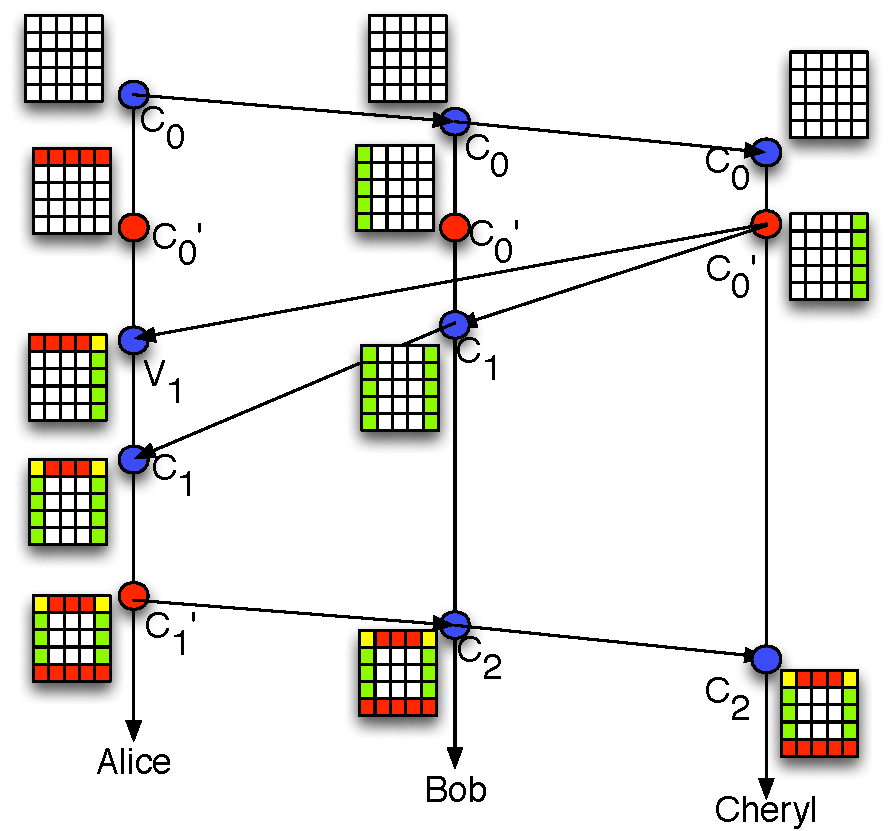
\includegraphics[scale=0.6]{Figures/canvas-sessions}
\caption{\drawsome: Collaborative drawing session visualized}
\label{fig:canvas-sessions}
\end{figure}
collaboration. All three of them start working on the blank canvas.
Alice draws a red horizontal line from $(0,0)$ (top-left) to $(4,0)$
(top-right) using \C{C.draw\_line}.\footnote{Its definitionis not
  shown, but can be constructed using \C{set\_px}} Meanwhile, Bob
draws a green vertical line from $(0,0)$ to $(0,4)$, and Cheryl draws
a similar line from $(4,0)$ to $(4,4)$. All three of them call
\C{sync} with their respective proposals ($C_0'$). While any partial
ordering of concurrent \C{syncs} is valid, we consider a linear order
where Cheryl's \C{sync} happens first, followed by Bob's and then
Alice's.  Cheryl's \C{sync} does not find any concurrent versions,
hence installs the proposed version ($C_0'$) as the next version on
Cheryl's branch. Bob's \C{sync} finds Cheryl's $C_0'$ as a concurrent
version, and merges it with its proposal to produce the next version
$C_1$, which is then installed on Bob's branch.  The least common
ancestor (LCA) for this merge is the initial version ($C_0$), and the
two concurrent versions are Bob's $C_0'$ and Cheryl's $C_0'$. Next,
Alice's \C{sync} finds Cheryl's $C_0'$ and Bob's $C_1$ as concurrent
versions, and merges them successively with Alice's proposal. For the
first merge, the two concurrent versions are Alice's $C_0'$ and
Cheryl's $C_0'$, and the LCA is the initial version ($C_0$). The
result of this merge is installed as the next version ($\C{V_1}$) on
Alice's branch. For the next merge, the two concurrent versions are
Alice's $V_1$ and Bob's $C_1$ and the LCA is Cheryl's
$C_0'$\footnote{Thus, the LCA of versions on two branches can lie
  outside both the branches.}. The result ($C_1$) becomes the next
version on Alice's branch, and the return value of Alice's \C{sync}.
Next, Alice draws a red horizontal line from $(0,4)$ to $(4,4)$,
proposes this canvas (\C{c1'} in the first column of
Fig.~\ref{fig:canvas-sessions-code}) as the next version to \C{sync}.
Since there are no concurrent versions, $C_1'$ becomes her next
version. The subsequent \C{sync} operations from Bob and Cheryl
propose no new versions, hence simply obtain Alice's $C_1'$ as next
versions.

The \drawsome example demonstrates the utility of mergeable data types
and \name programming model in building concurrent applications with
conceptual sharing of state. The model lets concurrent computations be
composed around any mergeable type. As exemplified by \drawsome,
writing a three-way \C{merge} function is the only creative process in
lifting an OCaml data type to a mergeable type. We now present few
more examples of mergeable types, and isolate a recurring pattern in
their merge functions that serves as a guide to write merge functions
for more sophisticated types.

\begin{figure}
  \centering
  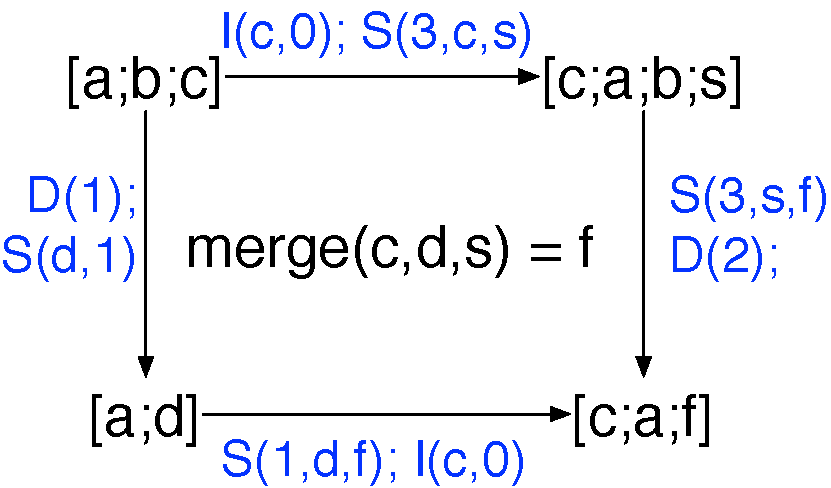
\includegraphics[scale=0.4]{Figures/list-eg}

  \caption{Lists of mergeable values are mergeable. }
  \label{fig:list-eg}
\end{figure}

\begin{figure}

\begin{subfigure}[b]{0.7\textwidth}
\begin{ocaml}
module type MList = sig
  module A: MERGEABLE
  include MERGEABLE
  type t = A.t list [@@deriving versioned]
  type edit = I of A.t * int
    | D of int
    | S of int * A.t * A.t
    | Nop
  ... (* All the standard list functions *)
  val insert: A.t -> int -> t -> t
  val delete: int -> t -> t
  val subst: int -> A.t -> t
  val edit_seq: t -> t -> edit list option
  val op_transform: edit list -> edit list -> edit list
  val merge: t -> t -> t -> t
end
\end{ocaml}
\caption{Signature of Mergeable Lists}
\label{fig:mlist-sig}
\end{subfigure}

\begin{subfigure}{0.75\textwidth}
\begin{ocaml}
(*
 * We reduce the problem of transforming op1* w.r.t op2* 
 * first to the problem of transforming op1* w.r.t op2,
 * and then to the problem of transforming op1 w.r.t op2.
*)
let op_transform mine others = 
  (*
   * Transforms my edit w.r.t other edit, and also returns how 
   * edits following my edit will witness the other edit.
   *)
  let xform my other = 
    let f my' = (my',other) in
    let g other' = (my,other') in
      match (my,other)  with 
      | (I (x,j), I (_,i)) when (j>=i) -> f @@ I (x,j+1)
      | (D j, I (_,i)) when (j>=i) -> f @@ D (j+1)
      | (S (j,x,y), I (_,i)) when (j>=i) -> f @@ S (j+1,x,y)
      | (I (x,j), D i) when (j=i) ->  g @@ Nop
      | (I (x,j), D i) when (j>i) ->  f @@ I (x,j-1)
      | (D j, D i) when (j=i) -> (Nop, Nop)
      | (D j, D i) when (j>i) ->  f @@ D (j-1)
      | (S (j,x,y), D i) when (j=i) -> f @@ Nop
      | (S (j,x,y), D i) when (j>i) -> f @@ S (j-1,x,y)
      | (I (x,j), S (i,y,z)) when (j<=i) -> g @@ S (i+1,y,z)
      | (D j, S (i,y,z)) when (j=i) -> g @@ Nop
      | (D j, S (i,y,z)) when (j<i) -> g @@ S (i-1,y,z)
      | (S (j,x,y), S (i,_,z)) when (j=i) -> f @@ S (j,x,A.merge x y z) 
      | _ -> f @@ my in
  let mine' = 
    List.fold_left 
      (fun mine other -> 
         let (mine',_) = 
           List.fold_left 
             (fun (xformed, other) my -> 
                let (my',other') = xform my other in
                  (xformed@[my'],other')) 
             ([],other) mine in
           mine') 
      mine others in
    mine'
\end{ocaml}
\caption{Operational transformation of list operations}
\label{fig:mlist-xform}
\end{subfigure}

\caption{Mergeable List Implementation}
\label{fig:mlist}
\end{figure}


{\bf Lists}. List, as an abstract data type, supports three
operations: \C{insert x i l}, that inserts an element \C{x} at
position \C{i} in the list \C{l}, \C{delete i l}, that deletes the
element at \C{i}'th position, and \C{subst i x l}, that substitutes
the element at \C{i}'th position with \C{x}. Lists of mergeable items
are mergeable. The signature of a mergeable list library is shown in
Fig.~\ref{fig:mlist-sig}. Note that the type of items in the list
(\C{A.t}) is also required to be mergeable. The signature
\C{MERGEABLE} will be discussed shortly. 

The merge operation for lists is composed of two separate functions,
\C{edit\_seq} and \C{op\_transform}.
\begin{itemize}
  \item \C{edit\_seq} takes a pair of lists, \C{v} and $\C{v'}$, and
  computes the shortest sequence of list operations that need to be
  applied on \C{v} to obtain \C{v'}. Such a sequence is called an
  \emph{edit sequence}. The length of the sequence corresponds to the
  standard notion of the \emph{edit distance} between the two lists,
  which can be computed in polynomial time, for e.g., using the
  Wagner-Fisher algorithm~\cite{wagner-fischer}. A slight modification
  of Wagner-Fischer also lets us compute the edit sequence. The
  implementation in Fig.~\ref{fig:mlist} represents edits using the
  type \C{edit}. Constructors \C{I}, \C{D}, and \C{S} stand for
  \C{insert}, \C{delete}, and \C{subst}, respectively; \C{Nop} is
  there for technical reasons. The subst constructor also carries the
  \C{A.t} element that was substituted. Our implementation of
  Wagner-Fischer is more-or-less standard (hence, not shown), except
  that the edit sequence it returns orders \C{I}'s and \C{D}'s before
  \C{S}'s.  Fig.~\ref{fig:list-eg} illustrates edit sequences for a
  sample list. The sequence \C{[I(c,0); S(3,c,s)]} maps the list
  \C{[a;b;c]} to \C{[c;a;b;s]} because \C{subst 3 s (insert c 0
  [a;b;c]) = [c;a;b;s]}.
  \item  \C{op\_transform} takes a pair of edit sequences, $s_1$ and
  $s_2$, that map a list $v$ to two different lists, $v_1$ and $v_2$
  (e.g., Fig.~\ref{fig:list-eg}), and transforms $s_1$ to $s_1'$ such
  that $s_1'$ has the same effect on $v_2$ as $s_1$ had on $v$.  For
  instance, in Fig.~\ref{list-eg}, let $s_1$ be the edit sequence
  \C{[D(1); S(d,1)]}, which maps the list \C{[a;b;c]} ($v$) to
  \C{[a;d]} ($v_1$). The \C{D} edit deletes the first element of $v$.
  However, if $s_1$ is to be applied on the list \C{[c;a;b;s]}
  ($v_2$), which has a new element at position 0, the \C{D} edit must
  delete the the second element from $v_2$, if it were to have the
  same effect as it did on $v$. We say \C{D(1)} in $s_1$ has to be
  transformed w.r.t the sequence $s_2 = \C{[I(c,0);S(3,c,s)]}$.  The
  function \C{op\_transform} of Fig.~\ref{fig:mlist-xform} computes
  such \emph{operational transformation} for the sequence \C{mine}
  w.r.t the sequence \C{others}, and returns \C{mine'} as the
  transformed sequence.  
\end{itemize}


This example, however, implicitly makes certain assumptions
about the model and the underlying system, such as the existence of a
single least common ancestor (LCA) for any pair of versions, the
ability to access a previous version on any branch, and mergeability
of any two concurrent versions. Enforcing these guarantees in a fully
decentralized distributed setting requires addressing non-trivial
theoretical challenges described in the next section. Unlike the
canvas, the process of writing merge functions for data types with
non-trivial invariants could be quite involved. The following sections
describe a principled approach to deriving merge functions for any
data type given its invariants. Like \C{Canvas.merge}, merge functions
often need to compare multiple versions of a data type for structural
equality, which, when performed naively, incurs cost linear in the
size of versions. The representation of a versioned data type in \name
is optimized for performing comparisons that allows structural
equality to be determined in constant time. Such engineering details,
which contribute to the practicality of our programming model are also
discussed in subsequent sections.



\section{Mergeable Types}
\label{sec:mergeable_types}

\begin{figure}

\begin{subfigure}{0.35\textwidth}
\begin{ocaml}
module type MRope = sig
  module A: sig
    type t
    val concat: t -> t -> t
    val split: t -> t*t
    val merge: t -> t -> t -> t
  end
  type t =
  | Leaf of A.t
  | Node of t * int * t
  ... 
  (* Standard rope functions *)
  val merge: t -> t -> t -> t 
end
\end{ocaml}
\caption{Signature of Mergeable Ropes}
\label{fig:mrope-sig}
\end{subfigure}
\begin{subfigure}{0.6\textwidth}
\begin{ocaml}
let rec flatten = function
  | Leaf x -> x
  | Node (l,_,r) -> A.concat (flatten l) (flatten r)

let rec merge old l r =
  if l = r then l else if old = l then r
  else if old = r then l else merge_rec old l r

and merge_rec old l r = match (old,l,r) with
  | Leaf _, _, _ | _, Leaf _, _ 
  | _, _, Leaf _ -> 
      rope_of @@ A.merge (flatten old) 
                    (flatten l) (flatten r)
  | Node (oldl,_,oldr), Node (ll,_,lr), 
    Node (rl,_,rr) ->
      let newl = merge oldl ll rl in
      let newr = merge oldr lr rr in
        Node (newl, create_index newl, newr)
\end{ocaml}
\caption{Mergeable rope implementation}
\label{fig:mrope-merge}
\end{subfigure}

\caption{Signature and implementation for mergeable ropes}
\label{fig:rope}
\end{figure}


The \drawsome example demonstrates the utility of the \name
programming model in building concurrent applications with conceptual
state sharing that make them suitable for transparent deployment in a
distributed setting. The model allows concurrent computations to be
composed around any mergeable type. We now present a series of
examples that demonstrate how mergeable types are built: either by
defining merge functions for ML data types, or by composing existing
mergeable types.

\subsection{Ropes}
\ref{sec:ropes}

A rope is a data structure that faciliates efficient implementations
of operations such as concatenation, splitting, lookup and insertion
at a random position etc., for a list of values in a distributed
setting. The values are usually characters, with their lists being
strings. The data structure is a binary tree, whose leaf nodes store
substrings of a larger string such that their left-to-right (in-order)
concatenation yeilds the larger string. The idea is to facilitate
efficient lookups and insertions at random positions in the string by
storing position indexes in the internal nodes of the tree.

Fig.~\ref{fig:mrope-sig} shows a rope interface in OCaml. The type of
the list of values is left abstract (\C{A.t}); it can be instantiated
with any module that supports \C{concat} and \C{split} operations. The
interface shown in Fig.~\ref{fig:mrope-sig} is that of a mergeable
rope (\C{MRope}), whose \C{merge} implementation is shown in
Fig.~\ref{fig:mrope-merge}. The function returns one of its versions
(\C{l} or \C{r}), if the other one is the same as the common
ancestor. Otherwise, it calls \C{merge\_rec}, which recursively
compares the structures of merging ropes, and their common ancestor.
The function recurses until one of the ropes differs from the other
two, or all of them are leaf nodes, at which point it relies on the
(abstract) list merge function (\C{A.merge}) to merge the lists
represented by the ropes. \C{merge\_rec} uses auxiliary functions,
\C{mk\_rope} and \C{create\_index}, whose definitions are not shown to
construct a rope given a list (\C{A.t}), and to compute the index at a
node, given its left sub-tree, resp.

One feature of the mergeable rope implementation that is characterisic
of mergeable types in general is compositionality; a rope is a
polymorphic mergeable data type that composes mergeability over its
polymorphic constituents.   Compositionality is concretized by the
\C{MRope} signature , which requires the type of items in the list
(\C{A.t}) to also be mergeable (\C{A.merge}).

\subsection{Lists}
\label{sec:lists}

\begin{figure}

\begin{subfigure}[b]{0.7\textwidth}
\begin{ocaml}
module type MList = sig
  module A: sig
    type t
    val merge: t -> t -> t -> t
  end
  type t = A.t list
  ... (* All the standard list functions *)
  val merge: t -> t -> t -> t (* and the merge function *)
  (* The following are exposed only for this presentation *)
  type edit = I of A.t * int
    | D of int
    | S of int * A.t * A.t
  val edit_seq: t -> t -> edit list option
  val op_transform: edit list -> edit list -> edit list
end
\end{ocaml}
\caption{Signature of Mergeable Lists}
\label{fig:mlist-sig}
\end{subfigure}


\caption{Mergeable List Implementation}
\label{fig:mlist}
\end{figure}


As an abstract data type, lists support three operations: \C{insert x
  i l}, to insert an element \C{x} at position \C{i} in the list
\C{l}, \C{delete i l}, to delete the element at \C{i}'th position, and
\C{subst i x l}, to substitute the element at the \C{i}'th position
with \C{x}.  Lists of mergeable items are mergeable if they preserve
the following properties:
\begin{itemize}
  \item Elements present in both the merging lists will be present in
  the final list. No element is deleted unless it is deleted in at
  least one list.
  \item An element deleted in one list will not reappear in the merged
  list (unlike, for example, Amazon's replicated shopping cart~\cite{Dynamo}).
  \item The order of elements is retained. That is, if $x$ occurs
  before $y$ in one of the lists, and if both elements are present in
  the merged list, then $x$ occurs before $y$ in the merged list.
\item If an element $y$ is substituted for an element $x$ in one list,
  then $y$ is also substituted for $x$ in the merged list (i.e., $x$
  is absent and $y$ is present), unless $x$ is deleted or substituted
  in the other list. In the former case, deletion wins, and neither
  $x$ nor $y$ occur in the merged list. In the latter case, if $x$ is
  substituted by a different element $z$ in the other list, then the
  merged list substitutes $x$ by a merge of $y$ and $z$, defined as
  per the merge semantics of the list element type.
\end{itemize}

\noindent The merge operation for lists is composed of two separate functions,
\C{edit\_seq} and \C{op\_transform}. Both these functions have been
implemented in less than 50 lines of OCaml included in the appendix.
The functions are described below.
\begin{itemize}
	\item \C{edit\_seq} takes a pair of lists, \C{v} and $\C{v'}$, and computes
		the shortest sequence of list operations that need to be applied on \C{v}
		to obtain \C{v'}. Such a sequence is called an \emph{edit sequence}. The
		length of the sequence corresponds to the standard notion of the \emph{edit
		distance} between the two lists, which can be computed in polynomial
		time~\cite{wagner-fischer}.  \C{edit\_seq} modifies one such algorithm to
		also compute the edit sequence (an \C{edit list}). The implementation
		specified in Fig.~\ref{fig:mlist-sig} represents edits using the type
		\C{edit}.  Constructors \C{I}, \C{D}, and \C{S} stand for \C{insert},
		\C{delete}, and \C{subst}, respectively.\footnote{ Note that \C{I}, \C{D}
		and \C{S} are \emph{not} effects; no list function generates them, and
		they are not exchanged between concurrent threads. They are simply tags
		used by the list merge operation for convenience.  Indeed, to better
		appreciate the virtues of mergeable types, we encourage the reader to
		think about how one might implement a replicated list with this
		functionality using an explicit effect representation as described in
		Sec.~\ref{sec:intro}.}  The subst constructor also carries the \C{A.t}
		element that was substituted. The element serves as the \C{lca} argument to
		\C{A.merge} in case of concurrent conflicting substitutions.
		Fig.~\ref{fig:list-eg} illustrates edit sequences for a sample list.  The
		sequence \C{[I(c,0); S(3,c,s)]} maps the list \C{[a;b;c]} to \C{[c;a;b;s]}
		because \C{subst 3 s (insert c 0 [a;b;c]) = [c;a;b;s]}.
	\item  \C{op\_transform} takes a pair of edit sequences, $s_1$ and $s_2$,
		that map a list $v$ to two different lists, $v_1$ and $v_2$ (e.g.,
		Fig.~\ref{fig:list-eg}), and transforms $s_1$ to $s_1'$ such that $s_1'$
		has the same effect on $v_2$ as $s_1$ had on $v$.  For instance, in
		Fig.~\ref{list-eg}, let $s_1$ be the edit sequence \C{[D(1); S(1,c,d)]},
		which maps the list \C{[a;b;c]} ($v$) to \C{[a;d]} ($v_1$). The \C{D} edit
		deletes the first element of $v$. However, if $s_1$ is to be applied on the
		list \C{[c;a;b;s]} ($v_2$), which has a new element at position 0, the
		\C{D} edit must delete the second element from $v_2$, if it were to
		have the same effect as it did on $v$. We say \C{D(1)} in $s_1$ has to be
		transformed w.r.t the sequence $s_2 = \C{[I(c,0);S(3,c,s)]}$.  The function
		\C{op\_transform} (Fig.~\ref{fig:mlist-sig}) computes such
		\emph{operational transformations} for an edit sequence $s_1$ w.r.t another
		edit sequence $s_2$. A notable transformation rule is for a substitution
		w.r.t another substitution at the same position. Since the substituting
		items could be different, the function relies on the item merge function
		(\C{A.merge}) to merge them into a single item. For instance, in
		Fig.~\ref{fig:list-eg}, there are simultaneous substitutions to the item
		\C{c} in $s_1$ and $s_2$; while $s_1$ substitutes it with \C{d}, $s_2$ does
		it with \C{s}. The merged list therefore substitutes \C{c} with the merge
		of \C{d} and \C{s}, defined as per the merge semantics of \C{A.t}.
\end{itemize}
The \C{MList.merge} can now be defined as a function that first
computes edit sequences, $s_1$ and $s_2$, for the two concurrent
lists, $v_1$ and $v_2$ w.r.t their common ancestor $v$, transforms one
of them (say, $s_1$) w.r.t $s_2$ to obtain $s_1'$, and finally applies
(the operations defined by) $s_1'$ to $v_2$ to obtain the merged list.

\subsection{Lists of Integers and Quantities}.

A mergeable list of integers can be composed using mergeable lists and
mergeable integers.  Concretely, it is a composition of \C{MList} and
\C{Int} types (i.e., \C{MList(Int)}), where \C{Int.merge} is the same
as \C{Counter.merge} (Sec.~\ref{sec:intro}).  An alternative
instantiation of \C{MList} is for a quantity type
(\C{Qty}) that supports \C{add} and \C{subtract} operations, but
\begin{wrapfigure}{l}{.45\textwidth}
  \centering
  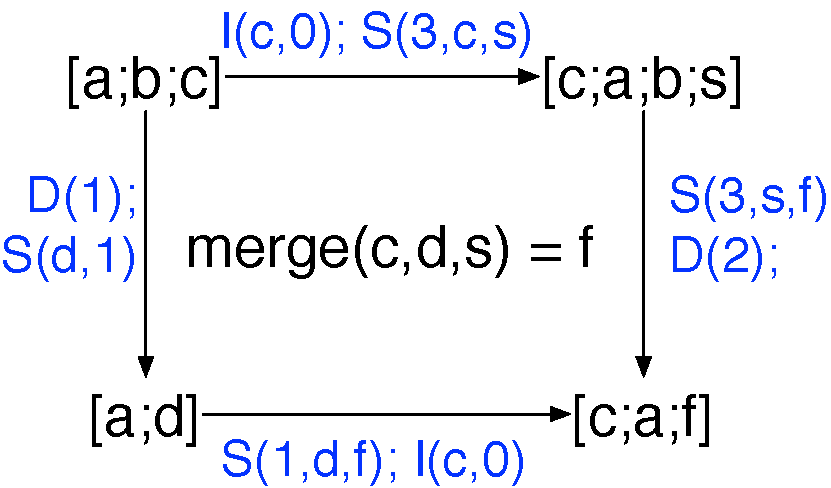
\includegraphics[scale=0.4]{Figures/list-eg}
  \caption{Lists of mergeable values are mergeable. }
  \label{fig:list-eg}
  \vspace*{-.2in}
\end{wrapfigure}
defines its \C{merge} opeation a little differently:
\begin{ocaml}
let merge lca v1 v2 = if v1 = lca then v2
    else (if v2 = lca then v1 else max v1 v2)
\end{ocaml}
\C{MList(Qty)}, like \C{MList(Int)}, is a list of integers, and has
the same semantics under a sequential execution. Their differences
however manifest under a concurrent execution, where both adopt
different methods to reconcile concurrent updates.

If efficient insertions and lookups (by position) are desired over a
large list of integers, while admitting concurrent updates, we require
a mergeable rope of integers, which can be obtained by simply
composing \C{MList(Int)} with \C{MRope} (i.e., \C{MRope(MList(Int))}).

% The mergeable list data type demonstrates a common pattern of writing
% \C{merge} functions applicable to a range of functional data
% structures. For instance, a binary tree (with rotations) can be made
% mergeable in the same way as list, i.e., by computing edit sequences
% (\C{edit\_seq}) and then their transformations
% (\C{op\_transform})\footnote{
%   Like Wagner-Fischer, established algorithms exist for computing tree
%   edit distances~\cite{tree-diff}. An alternative naive method to
%   merge a pair of trees is by merging the lists obtained from their
%   in-order traversal, followed by reconstructing the tree.
% }.

\subsection{Shopping List}

\begin{figure}
\centering
\begin{tabular}{l||l}
\begin{ocaml}
let alice_f : L.t unit t =
  fork bob_f >>= fun () -> (* Invite Bob *)
  get () >>= fun c0 ->
  let qty = L.assoc "eggs" in
  let c0' = L.subst 1 ("eggs",qty+1) c0 in
  sync () ~v:c0' >>=
  fun c1 -> return ()
\end{ocaml}
&
\begin{ocaml}
let bob_f : L.t unit t =
  get () >>= fun c0 ->
  let c0' = L.insert ("candy",Qty.of_int 1) 1 @@
            L.delete @@ L.lookup "eggs" in
  sync () ~v:c0' >>=
  fun c1 -> return ()
\end{ocaml}
\\
\end{tabular}
\caption{Bob and Alice collaboratively build a grocery shopping list}
\label{fig:shopping-list-code}
\end{figure}

A non-trivial demonstration illustrating the compositional power of
mergeable types is shopping list application, that allows its users to
collaboratively build a shopping list (listing items in the decreasing
order of their priority), by adding new items with a
specified quantity, deleting existing items, and increasing or
\begin{wrapfigure}{l}{.5\textwidth}
  \centering
  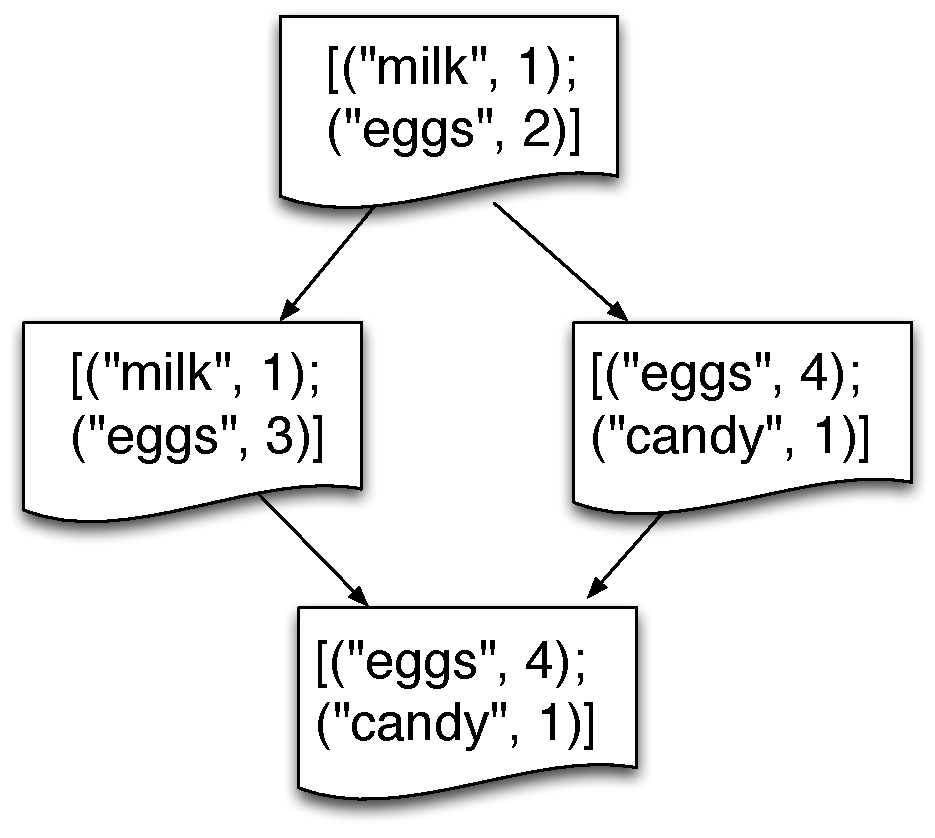
\includegraphics[scale=0.3]{Figures/shopping-list}
  \caption{Merging concurrent shopping lists}
  \label{fig:shopping-list}
  \vspace*{-.2in}
\end{wrapfigure}
decreasing their quantity. An item (\C{Item.t}) is represented as a
tuple of its name (a string) and the quantity (A \C{Qty.t}). The merge
function for \C{Item.t} merges the quantities of items (using
\C{Qty.merge}) having the same names. Items with different names are
considered distinct. A shopping list is a mergeable list of items,
i.e., \C{MList(Item)} (a grocery shopping list may not be large enough
to justify using ropes, but \C{MRope(MList(Item))} is definitely a
possibility).  \C{MList(Item).merge} automatically lifts the merge
semantics for items to merge semantics for lists of items.
Fig.~\ref{fig:shopping-list} illustrates its behavior.  Here, two
users, Alice and Bob, concurrently edit a shopping list whose initial
contents are \C{milk} and \C{eggs}. While both simultaneously update
the quantity of eggs, Bob also removes \C{milk} and inserts \C{candy}.
Fig.~\ref{fig:shopping-list-code} shows the \name code for two
concurrent sessions. The merged shopping list contains \C{eggs} and
\C{candy}, where the quantity of eggs is obtained by merging Alice's
and Bob's quantity as per the definition of \C{Qty.merge}.

The examples described above make certain assumptions about the model
and the underlying system, such as the existence of a single least
common ancestor (LCA) for any pair of versions, the ability to access
a previous version on any branch, and mergeability of any two
concurrent versions. Enforcing these guarantees in a fully
decentralized distributed setting requires addressing non-trivial
theoretical challenges. These, and other details that contribute to
the practicality of our model, such as containing the complexity of
merges, are discussed in subsequent sections.




\section{Operational Semantics}

\begin{figure*}[!t]
\raggedright
%
\textbf{Syntax}\\
%
\begin{smathpar}
\renewcommand{\arraystretch}{1.2}
\begin{array}{lclcl}
\multicolumn{5}{c} {
  t \in \mathtt{Thread\; Ids} \qquad
  x,y \in \mathtt{Variables} \qquad
  c \in \mathtt{\{()\}} \cup \mathbb{N} \qquad
}\\
v & \in & \mathtt{Values} & \coloneqq & c \ALT \lambda x.\,s\\
s & \in & \mathtt{Expressions} & \coloneqq & v \ALT s\;s \ALT \run{s}{s}
   \ALT \fork{s} \ALT \pull \ALT \push{s}\\
p & \in & \mathtt{Programs} & \coloneqq & s_t \ALT p\,||\,p \\
f & \in & \mathtt{Tags} & \coloneqq & \C{INIT} \ALT \C{FORK} \;b 
  \ALT \C{PUSH} \ALT \C{MERGE} \;b\\
b & \in & \mathtt{Branches} & \coloneqq & [(v,f)] \ALT (v,f)::b \\
\end{array}
\end{smathpar}
%
\bigskip
%% If we are feeling adventurous, we can try defining e and s 
%% mutually recursively, such that their evaluation relations 
%% are also mutually recursive (multiple reduction steps of one 
%% relation is a single step of other). 

%
\textbf{Evaluation Contexts}\\
%
\begin{smathpar}
\renewcommand{\arraystretch}{1.2}
\begin{array}{lclcl}
H & \in & \mathtt{Branch\; Histories} & \coloneqq & t \mapsto b\\
E & \in & \mathtt{Eval.\; Contexts}(s) & \coloneqq & \bullet \ALT 
  \bullet\;s \ALT v\;\bullet \ALT \run{\bullet}{s}\\
P & \in & \mathtt{Eval.\; Contexts}(p) & \coloneqq & E_t \ALT 
  \bullet\,||\,p \ALT p\,||\,\bullet \\
\end{array}
\end{smathpar}
%
\bigskip

%
\textbf{Reduction Relation} \quad \fbox {$p;\;H \stepsto p';\;H'$} \\
%
%
\begin{smathpar}
\begin{array}{lcll}
(\run{v}{s})_t;\cdot & \stepsto & 
  s_t; \cdot[t_{\top} \mapsto [(v,\C{INIT})]]
            [t\mapsto [(v,\C{FORK}\; [(v,\C{INIT})])]] 
            & [\rulelabel{E-Run}]\\
(\fork{s})_t;H(t\mapsto (v,\_)::b) & \stepsto & 
    ()_t\,||\, s_{t'}; H[t'\mapsto [(v, \C{FORK} H(t))]] 
    \spc \texttt{where}\; t'\not\in dom(H)
            & [\rulelabel{E-Fork}]\\
(\push{v})_t;H & \stepsto & ()_t;H[t \mapsto (v,\C{PUSH})::H(t)]
            & [\rulelabel{E-Push}]\\
% & & & v\,=\,\C{merge}\,v\,v_1\,v_2 ~\texttt{and}~ \\
((\lambda x.s)\;v)_t;H & \stepsto & ([v/x]\,s)_t;H
            & [\rulelabel{E-App}]\\
(\pull)_t;H(t \mapsto (v,\_)::m) & \stepsto & v_t;H
            & [\rulelabel{E-Pull}]\\
\end{array}
\end{smathpar}
%

% %
% \hspace*{\fill}[\rulelabel{E-Admin}]\hspace*{0.25in}
% \begin{smathpar}
% \begin{array}{c}
% \RULE
% {
%   s_t; H ~\stepsto^{*}~ v_t; H
% }
% {
%   E_t[s]; H ~\stepsto^{*}~ E_t[v]; H
% }
% \end{array}
% \end{smathpar}
% %

%
\hspace*{\fill}[\rulelabel{E-Pull-Wait}]
\begin{smathpar}
\begin{array}{c}
\RULE
{
  t\neq t' \spc
  \under{H}{v' \mbleto v} \spc
% \C{world}(H,t') \semsucceq \C{world}(H,t)\spc 
  v_m = \C{merge}(\C{lca}(H(t),H(t')), v, v') \spc
}
{
  (\pull)_t;H(t \mapsto (v,f)::m)(t' \mapsto (v',\_)::\_) ~\stepsto~
  (\pull)_t;H[t \mapsto (v_m,\C{MERGE}\; H(t'))::(v,f)::m]
}
\end{array}
\end{smathpar}
%

\caption{\name: Syntax and Operational Semantics}
\label{fig:opsem}
\end{figure*}


We formalize our ideas in the context of a lambda calculus ($\lang$)
shown in Fig.~\ref{fig:opsem}. Expressions of $\lang$ are variables,
constants, and \name primitives composed using the lambda combinator.
For brevity, we use short names for \name primitives: \C{run} for
\C{with\_init\_version\_do}, and \C{fork} for \C{fork\_version}. To
simplify the technical development, \name's \C{sync\_next\_version}
operation is broken down into two primitives - \C{push} and \C{pull},
which can be lambda-composed get the desired effect:
\begin{smathpar}
  \C{sync}\;x \;=\; (\lambda y.\pull)\; (\push\,x)
\end{smathpar}
The semantics of\C{get\_current\_version} is subsumed by \C{pull},
hence elided.  Values ($v$) are constants and lambda abstractions.  A
program ($p$) is a parallel composition of threads, where each thread
is an expression ($s$) indexed by the corresponding thread identifier
($t$). 

Fig.~\ref{fig:opsem} also shows the syntax of \emph{branches}, which
are the artifacts of evaluation and only appear during the run-time. A
branch is a non-empty sequence of tagged values, where the tag
captures the abstract run-time operation that led to the creation of
the value. It is implicitly assumed that each value added to a branch
is uniquely identifiably, hence no two values on a branch are equal.
The uniqueness assumption is later extended to a collection of
branches that constitute a branching structure. A real implementation
meets this assumption by versioning values across the branches. Thus,
in reality, branches contain \emph{versions} which denote values. The
semantics, however, doesn't make this distinction, and uses values and
versions interchangeably.

Small-step operational semantics of $\lang$ is defined via reduction
relation ($\stepsto$) that relates \emph{program states}. A program
state ($p;\,H$) consists of a program $p$ and a \emph{branch history}
$H$ that maps thread Ids to corresponding branches; each thread is
associated with a branch during the evaluation. Evaluation contexts
have been defined separately for expressions ($E$) and programs ($P$),
with the latter subsuming the former. $E$ is defined to evaluate the
first argument of a \C{run} expression to a value that constitutes the
initial version (recall that \C{run} models \name's
\C{with\_init\_version\_do}). Program evaluation context
non-deterministically picks one of the threads to evaluate. The admin
rule that relates transitions of holes to transitions of expressions
and programs is straightforward, hence elided. Rest of the reduction
rules are presented in Fig.~\ref{fig:opsem}. For brevity, we write
$H(t\mapsto (v,f))$ to denote the proposition that $H$ maps $t$ to
$(v,f)$. The notation $H[t \mapsto (v,f)]$ as usual denotes
the extension of $H$ with the binding $t \mapsto (v,f)$.

Reduction rules let expression evaluation take a step by rewriting the
expression and suitably updating the branch history ($H$). The
\rulelabel{E-Run} rule is applicable only when $H$ is empty, i.e.,
when no prior branching structure exists. The rule rewrites the
$\C{run}\;v\;s$ expression to $s$, while creating a new branching
structure with two branches: a \emph{top} branch that has just the
initial version (tagged with \C{INIT}), and a branch for the current
thread ($t$) forked-off from the top branch.  The first version on the
current branch ($H(t)$) denotes the same value ($v$) as the initial
version on the top branch, although versions themselves are deemed
distinct. The new version is tagged with a \C{FORK} tag that keeps the
record of its orgin, namely the \C{fork} operation and the branch from
which the current branch is forked. The \rulelabel{E-Fork} rule forks
a new thread with a fresh id ($t'$) and adds it to the thread pool.
The corresponding branch ($H(t')$) is forked from the parent thread's
branch ($H(t)$). The semantics of branch forking is same as described
above. The \C{fork} expression in the parent thread evaluates to
\C{()}. The \rulelabel{E-Push} rule creates a new version on the
current branch ($H(t)$) using the pushed value ($v$).
\rulelabel{E-App} is the standard beta reduction rule.

The semantics non-deterministically chooses \rulelabel{E-Pull} or
\rulelabel{E-Pull-Wait} rules to reduce a \C{pull} expression. The
\rulelabel{E-Pull} rule reduces \C{pull} to \C{()}, and returns the
latest version on the current branch. The \rulelabel{E-Pull-Wait} rule
can be thought of as a stutter step; it doesn't reduce \C{pull}, but
updates the branching structure by merging (the latest version of) a
concurrent branch ($H(t')$) into (the latest version of) the current
branch ($H(t)$), and extending the current branch with the merged
version ($v_m$). The new version is tagged with a \C{MERGE} tag that,
like a \C{FORK} tag, records its origin. The premises of the
\rulelabel{E-Pull-Wait} serve the important purpose of contraining the
branching structure by allowing only the legal merges, and
consequently preserving certain desirable properties of the system;
we will go into the details shortly. The \rulelabel{E-Pull-Wait} and
\rulelabel{E-Pull} rules thus let a thread sync with a subset of
concurrent threads in multiple steps before returning the result of
the \C{pull}. Since \C{sync} is a composition of \C{push} and
\C{pull}, its behavior can be explained thus: \C{sync} pushes the
given value onto the current (local) branch, merges a (possibly empty)
subset of concurrent branches into the local branch, and returns the
result.

We will now present a series of definitions and results that let us
understand the premises of the \rulelabel{E-Pull-Wait} rule, examine
the merge operation in closer detail, and appreciate the need for
constraining the branching structure. First, we formalize the
intuitive notation of the ancestor relationship between versions of a
legal branching history (i.e., a branching history generated by the
rules in Fig.~\ref{fig:opsem}):

\begin{definition} [\bfseries Ancestor]
Version $v_1$ is a ancestor of version $v_2$ under a history
$H$ (written $\under{H}{v_1 \preceq v_2}$) if and only if one of the
following is true:
\begin{itemize}
  \item There exists a branch $b$ in $H$ (i.e., $\exists(t\in
  dom(H)).\,H(t) = b$) in which $v_2$ immediately succeeds
  $v_1$,
  \item There exists a branch $b$ in $H$ that contains $(v_2, 
  \C{FORK}\; (v_1,f_1)::b_1)$, for some $f_1$ and $b_1$,
  \item There exists a branch $b$ in $H$ that contains
  $(v_2, \C{MERGE}\;(v_1,f_1)::b_1)$, for some $f_1$ and $b_1$,
  \item $v_1 = v_2$, or $v_1$ is transitively a ancestor of
  $v_2$, i.e., $\exists v.~ \under{H}{v_1 \preceq v} \conj
  \under{H}{v \preceq v}$ 
\end{itemize}
\end{definition}

Ancestor relation is therefore a partial order (reflexive, transitive,
anti-symmetric) with a greatest lower bound (the initial version).
Thus, for any two versions in a legal history, there exist at least
one common ancestor. Ancestor relationships among the common ancestors
let us define the notion of a least common ancestor (LCA):

\begin{definition} [\bfseries Least Common Ancestor]
Version $v$ is said to be a common ancestor of versions $v_1$ and
$v_2$ under a history $H$ if and only if $\under{H}{v \preceq v_1}$
and $\under{H}{v \preceq v_2}$. It is said to be the least common
ancestor (LCA) of $v_1$ and $v_2$, iff there does not exist a $v'$
such that $\under{H}{v' \preceq v_1}$ and $\under{H}{v' \preceq v_2}$
and $\under{H}{v \preceq v'}$.
\end{definition}

\begin{figure}
\centering
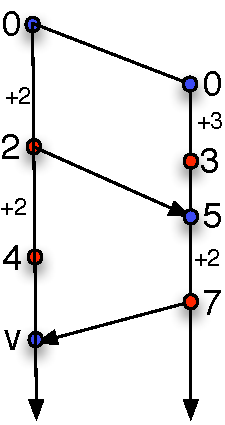
\includegraphics[scale=0.6]{Figures/merge-needs-lca}

\caption{This example of a grow-only counter illustrate why \C{merge}
needs a least common ancestor, and not just a common ancestor. Both 0
and 2 are common ancestors of 4 and 7, while 2 is their least common
ancestor (since $0 \preceq 2$). The result (v) of merging 4 and 7 is
11 (incorrect) if 0 is used as the common ancestor for merge, and 9
(correct, because 2+2+3+2 = 9) if 2 is used. }
\label{fig:merge-needs-lca}
\end{figure}

\begin{figure}[!t]
\centering
\subcaptionbox[] {\small
  In this example, 1 and 3 have two LCAs (3 and 4) a result of
  previous merges. The dotted circle denotes a virtual ancestor
  obtained by merging the two LCAs.
  \label{fig:criss-cross-lcas}
} [0.47\columnwidth] {
  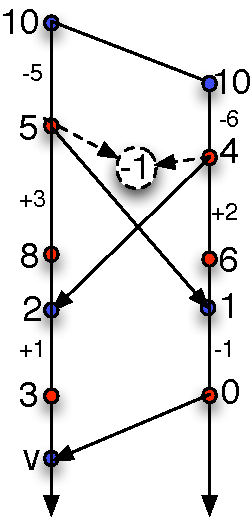
\includegraphics[scale=0.55]{Figures/2-LCAs}
}
\hfill
\subcaptionbox[] {\small
  In this example, 3 and 6 have two LCAs (2 and 1) despite there not
  being any previous merges between their respective branches.
  \label{fig:external-lcas}
} [0.47\columnwidth] {
  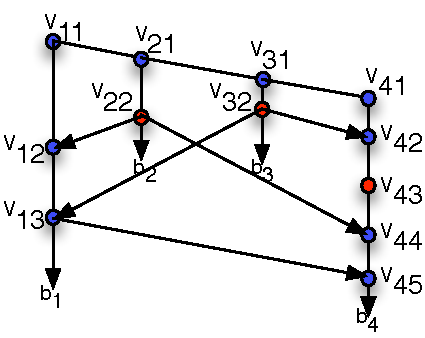
\includegraphics[scale=0.7]{Figures/2-external-LCAs}
}
\caption{Examples where merging versions have more than one LCA}
\label{fig:many-lcas}
\end{figure}

When merging two concurrent versions $v_1$ and $v_2$, the common
ancestor argument for \C{merge} must the LCA of $v_1$ and $v_2$,
without which \C{merge} may yeild unexpected results. This is
demonstrated for the grow-only counter in
Fig.~\ref{fig:merge-needs-lca}, where incorrect count is obtained if a
common ancestor that is not an LCA is used to merge 4 and 7. While in
this example there is a unique LCA for 4 and 7, in general this may
not be the case. With unrestrained branching and merging, there is no
bound on the number of LCAs a pair of versions can have.
For example, in
Fig.~\ref{fig:criss-cross-lcas}, the merge of 0 with 3 is preceded by
two ``criss-cross'' merges between their respective branches resulting
in there being two LCAs (5 and 4) for 0 and 3. Multiple LCAs can occur
even without criss-cross merges, as demonstrated by
Fig.~\ref{fig:external-lcas}. The problem with concurrent versions
with multiple LCAs is that they do not lend themselves to three-way
merging. This problem also arises in the context of source
control systems, and often solved via ad-hoc mechanisms.
GitHub~\cite{github}, for instance, recursively merges LCAs to compute
a virtual ancestor, which then serves as the LCA for merging the
concurrent versions. This method is demonstrated for the example in
Fig.~\ref{fig:criss-cross-lcas}, where LCAs 5 and 4 of 0 and 3 are
merged (with LCA of 10) to generate -1 as the virtual LCA to merge 5
and 4. A major downside with this method is that it makes no
guarantees of the relationship between the virtual ancestor and the
concurrent versions; the former may not even be a legal ancestor of
the latter as per the semantics of the data type. For instance, the
integer type in Fig.~\ref{fig:criss-cross-lcas} may in fact represent
a bank account, which disallows any activity on the account if balance
is ever known to be less than zero. Thus, from the perspective of a
bank account, it doesn't make sense how concurrent versions 3 and 0
emerged from -1, since the only transition allowed by the semantics
from -1 is to itself. Clearly, ad hoc mechanisms, which work for the
text, may not work for more sophisticated data types.

Fortunately, unlike the source control systems where branching
structure is entirely dictated by the user, \name abstracts away the
branching structure from the programmer, hence retains the ability to
constrain it in a way that it deems fit. In particular, \name solves
the problem of multiple LCAs by suitably constraining the branching
structure such that the problem never arises. The constraints are
imposed either implicitly, as a result of how operational semantics
defines an atomic step, or explicitly, by insisting that certain
conditions be met before merging a pair of versions
(\rulelabel{E-Pull-Wait}). Firstly, the operational semantics already
disables criss-cross merges since it only ever merges versions that
are latest on their respective branches. For instance let $v_{11}$ and
$v_{21}$ be the latest versions on branches $b_1$ and $b_2$,
respectively. Meging $b_2$ into $b_1$ requires entails $v_{21}$ into
$v_{11}$ to generate version $v_{12}$ on $b_1$. Now, merging $b_1$
into $b_2$ translates to merging $v_{12}$ into $v_{21}$ (a
\emph{fast-forward} merge, in Git parlance), but not $v_{11}$ into
$v_{21}$, thus preventing a criss-cross branching structure. In other
words, a criss-cross branching structure is prevented due to the
order among merges between conflicting branches introduced as a result
of \rulelabel{E-Pull-Wait} being an atomic step. 

Secondly, we impose certain pre-conditions on the merging branches to
preempt the structure shown in Fig.~\ref{fig:external-lcas}. The
intuition is as follows: consider the branch $b_1$ at the instance of
merging $b_3$. Since it has already merged $b_2$, a version on $b_2$
($v_{22}$) could be a common ancestor for a version on $b_1$
($v_{12}$) and some other version (call it $v$). Now, if $b_1$ merges
$b_3$, same could be true of $b_3$ and $b_1$: a version on $b_3$
($v_{32}$) could be a common ancestor for the new version on $b_1$
($v_{13}$), and the other version $v$. Since $v_{22}$ is also an
ancestor of $v_{13}$, and both ancestors are not ordered by the
ancestor relation, $v_{13}$ and $v$ end up with two LCAs. In
Fig.~\ref{fig:external-lcas}, the role of $v$ is played by the version
$v_{44}$. We observe that this scenario can be prevented if, when
merging $b_3$, $b_1$ insists on an ancestor relation between the
merged version ($v_{22}$) of the $b_2$, the previously merged branch,
and the latest version of $b_3$, the current merging branch. We call
the last merged version the \emph{external locus} of the branch. By
requiring that, for every branch $b$, the external locii of $b$ at
various points in time (i.e., external locus of every prefix of $b$)
be totally ordered, we effectively enforce the invariant that for any
two common ancestors $v_1$ and $v_2$ between two versions, there
exists another common ancestor $v_3$ that succeeds $v_1$ and $v_3$ in
the ancestor relation, thereby preventing the possibility of multiple
LCAs.

%% <false>
%% Multiple versions that merge any pair of versions are totally
%% ordered. That is, if $v_1$ and $v_2$ are ancestors of $v_3$ and
%% $v_4$, then $v_3$ and $v_4$ are ordered by the ancestor relation.
%% </false>

%% If $v_1$ and $v_2$ are ancestors of $v_3$ and $v_4$, then there
%% exists a $v_5$, a successor of $v_1$ and $v_2$, and an ancestor of
%% $v_3$ and $v_4$
%% If I follow one of your locii, or you follow one of my locii, then
%% we both have same set of external common ancestors.

Let us see how the aforementioned restriction allows us to merge the
branches in Fig.~\ref{fig:external-lcas} without ever creating
multiple LCAs. The legal branching history is shown in
Fig.~\ref{fig:legal-merge}. First, like in
Fig.~\ref{fig:external-lcas}, $b_2$ is merged into $b_1$ to create
$v_{12}$, and $b_3$ is merged into $b_4$ to create $v_{42}$. Thus, the
external locus of $b_1$ is $v_{22}$, and that of $b_4$ is $v_{32}$.
Observe that now $b_1$ cannot merge $b_3$, neither can $b_4$ merge
$b_2$ because $v_{22}$ and $v_{32}$ are not related by the ancestor
relation. Same applies for $b_1$ and $b_4$ because neither one's
latest version follows from other's external locus.  However, $b_2$
and $b_3$ can merge among themselves. Let us say they indeed merge to
to create a version $v_{23}$ on $b_2$. The branch $b_2$ is now
eligible to be merged into $b_1$ and also $b_4$. These merges do occur
in Fig.~\ref{fig:legal-merge} to create versions $v_{13}$ and
$v_{43}$, and making $v_{23}$ the external locus for both $b_1$ and
$b_4$. Thus, $b_1$ can now merge into $b_4$ to create version $v_{44}$
on $b_4$.

We now formalize the intuitions described above to precisely define
the notion of mergeability:

\begin{definition} [\bfseries Internal and External Ancestors]
Given a branch $b$ and a version $v\in b$, an internal ancestor of $v$
is an ancestor from the same branch $b$. An external ancestor of $v$
is an ancestor from a different branch $b'\neq b$. 
\end{definition}

\begin{definition} [\bfseries External Locus]
Given a branch $b$ and a version $v\in b$, external locus ($v_o$) of
$v$ is an external ancestor that is not an ancestor of any other
external ancestor of $v$. That is, $\under{H}{v_o \preceq v}$, and
there does not exist a $v_o' \not\in b$ such that $\under{H}{v_o'
\preceq v}$ and $\under{H}{v_o \preceq v_o'}$. 
\end{definition}

\begin{definition} [\bfseries Mergeability]
Given a history $H$, a version $v_1$ and a version $v_2$ that is not
an ancestor of $v_1$ under $H$, $v_2$ is mergeable into $v_1$ (denoted
$\under{H}{v_2 \mbleto v_1}$) iff $v_1$'s external locus is an
ancestor of $v_2$, or $v_2$'s external locus is an ancestor of $v_1$.
\end{definition}

Rule \rulelabel{E-Pull-Wait} of the reduction relation
(Fig.~\ref{fig:opsem}) is enabled only if the latest version ($v'$)
of thread $t'$'s branch is mergeable into the latest version ($v$) of
thread $t$'s branch (i.e., $\under{H}{v' \mbleto v}$). Merge computes
the latest common ancestor of $v$ and $v'$, which is 
guaranteed to be unique as per the following theorem\footnote{Proof
included in the appendix}:

\begin{theorem} [\bfseries Unique LCA]
Every pair of versions $v_1$ and $v_2$ in a legal branch history $H$ 
have a unique least common ancestor. 
\end{theorem}

The \rulelabel{E-Pull-Wait} uses the function \C{lca} to compute the
LCA of (the latest versions on) a pair of branches. The definition of
the function is standard, hence not discussed.


\section{Distributed Instantiation}
\label{sec:implementation}

We describe the realization of \name on top of a persistent
distributed store and the language extensions to enable and enforce
the constraints of the \name.

The \name programming model is realized on top of Irmin~\cite{irmin},
an OCaml library database implementation that is part of the MirageOS
project~\cite{mirage}. Irmin provides a persistent multi-versioned
store with a content-addressable heap abstraction. Simply put,
content-addressability means that the address of a data block is
determined by its content. If the content changes, then so does the
address. Old content continues to be available from the old
address. Content-addressability also results in constant time
structural equality checks, which we exploit in our mergeable rope
implementation (Section~\ref{sec:ropes}), among others.

Irmin provides support for distribution, fault-tolerance and
concurrency control by incorporating the Git distributed version
control~\cite{git} protocol over its object model. Indeed, Irmin is
fully compatible with Git command line tools. Distributed replicas in
\name are created by cloning a \name repository. Due to \name's
support for mergeable types, each replica can operate completely
independently, accepting client requests, even when disconnected from
other replicas, resulting in a highly available distributed system.

\begin{wrapfigure}{L}{.5\textwidth}
	\begin{center}
	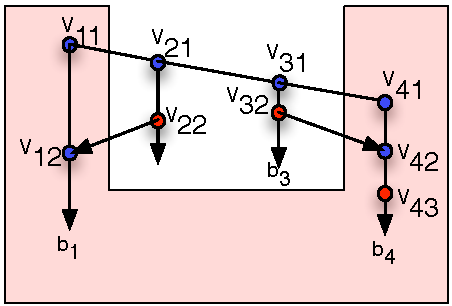
\includegraphics[scale=0.8]{Figures/partitions}
	\end{center}
  \caption{Network partitions may leave branches $b_1$ and $b_4$ in
  one partition (red background), and branches $b_2$ and $b_3$ in the
  other (yellow background). Access to full history on both sides of
  the partition lets both sides make progress.}
	\label{fig:partitions}
\end{wrapfigure}

Concurrent operations in Irmin are tracked using the notion of
branches, allowing the programmer to explicitly merge branches on
demand. \name's concurrency and distribution model is also realized in
terms of branches; each replica operates on its own branch, and thus
is isolated from the actions on other replicas. In the presence of
network partitions, the nodes in one partition may not receive updates
from the other partition, preventing merges from happening across a
partition. This can be a problem if a pair of branches in one
partition (the current partition) have multiple LCAs in the other
partition (the remote partition), and hence cannot
merge. Fig.~\ref{fig:partitions} illustrate this problem for the
branching structure of Fig.~\ref{fig:external-lcas}.

Fortunately, access to full (causal) branching history assured by
Irmin at every node comes to the rescue. Relying on the history, the
current partition can fork-off (\C{fork}) new branches that start
where the remote branches left, and map them to new (virtual) nodes
that emulate the nodes in the remote partition. For the example in
Fig.~\ref{fig:partitions}, the partition of $b_1$ and $b_4$ can fork
new branches $b_2'$ and $b_3'$ from $b_2$ and $b_3$, respectively, and
resume the activity as if the partition never happened. After merging
the first versions on $b_2'$ and $b_3'$, branches $b_1$ and $b_2$ will
be in the same state as before (when the partition happened), except
that the branches are now mergeable because $b_2'$ and $b_3'$ can
merge. The ability to track full provenance information is thus
crucial for \name to overcome network partitions, making it an
appropriate programming model for highly-available replicated data
types. The \nameMonad conceals branching structure, but also
transparently performs the necessary merges to obtain a history graph
with a unique lowest common ancestor.

Importantly, Irmin supports user-defined three-way merge functions for
reconciling concurrent operations. While Irmin's merge functions are
defined over objects on Irmin's content-addressable heap, \name's
merge functions are defined over OCaml types. We address this
representational mismatch with the help of OCaml's PPX metaprogramming
support~\cite{ppx} to derive bi-directional transformations between
objects on OCaml and Irmin heaps. We also derive the various
serialization functions required by Irmin\footnote{
  The Since \nameMonad monad relies on Irmin for realizing the branch
  structure, it is in fact parameterized over a mergeable type that
  implements all these functions. Thus the monad is functorized over
  the mergeable type, but not polymorphic. The convenience of type
  parameter inference that polymorphism offers can however be obtained
  for module parameters using OCaml extensioms, such as Modular
  Implicits~\cite{implicits}.
}.
Synchronization between replicas is performed using Git's notion of
pushing and pulling updates from remotes~\cite{git-tp}. As a result, we reap the
benefits of efficient delta-transfer (only missing objects are transferred between
replicas), compression and end-to-end encrypted communication between
the replicas.


\section{Evaluation}
\label{sec:evaluation}

In this section, we present an evaluation of \name programming model with the
aim of assessing its practical utility for describing geo-distributed
eventually consistent applications. In particular, we are interested in the
horizontal scalability of applications built using \name. Typical distributed
eventually consistent data stores use custom synchronization and dissemination
protocols for transferring updates between replicas. Unlike this, \name is
realized over Irmin which uses Git transfer protocol~\cite{..}, a protocol not designed
with distributed data stores in mind. Hence, we also evaluate the performance
of synchronization and merging.

\subsection{Benchmark: Collaborative editing}

In order to evaluate this, we have implemented a collaborative editing
application that simulates concurrent editing of the same document by several
authors. This application is not unlike Google Docs, but also differs from it
by the fact that we do not need a central server that coordinates the edits.
Instead, edits from each author is asynchronously sent to other authors. The
shared document itself is represented by a mergeable rope of characters
(Section~\ref{sec:model}), and hence, the remote edits can be correctly
reconciled into the local document. We resolve conflicts on concurrent
substitutions at the same position (such as two authors concurrently editing
\C{"abc"} to \C{"xbc"} and \C{"ybc"}, respectively) by choosing the character
with the smaller ASCII code. For the benchmarks, the initial document that we
use has 1576 characters. The workload consists of 4000 edit operations at
random indices with 85\% insertions and 15\% deletions.

\subsection{Experimental setup}

\begin{figure}[t]
  \centering
	\begin{subfigure}{0.45\textwidth}
		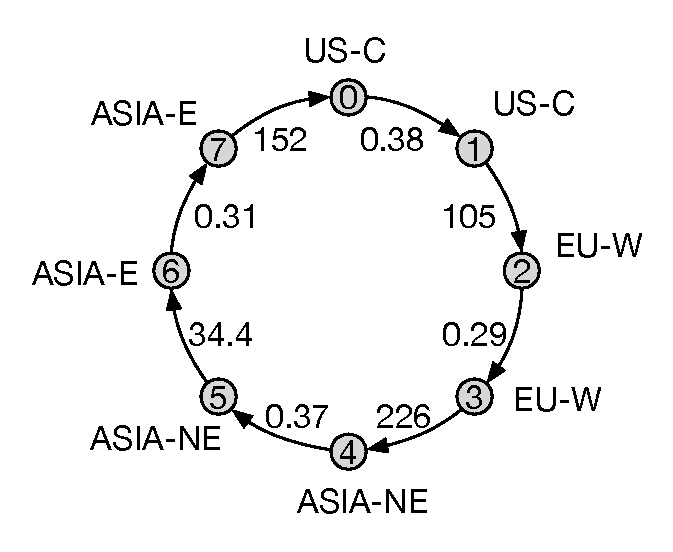
\includegraphics[width=0.9\textwidth]{Figures/cluster.pdf}
		\caption{8-node ring cluster on Google Cloud Platform used for
			benchmarking. US-C, EU-W, ASIA-NE and ASIA-E are availability zones
			us-central1-b, europe-west1-b, asia-northeast1-b and asia-east1-b
			respectively. Edge labels are inter-node latencies in milliseconds.}
		\label{fig:cluster}
	\end{subfigure}
	\hfill
	\begin{subfigure}{0.45\textwidth}
		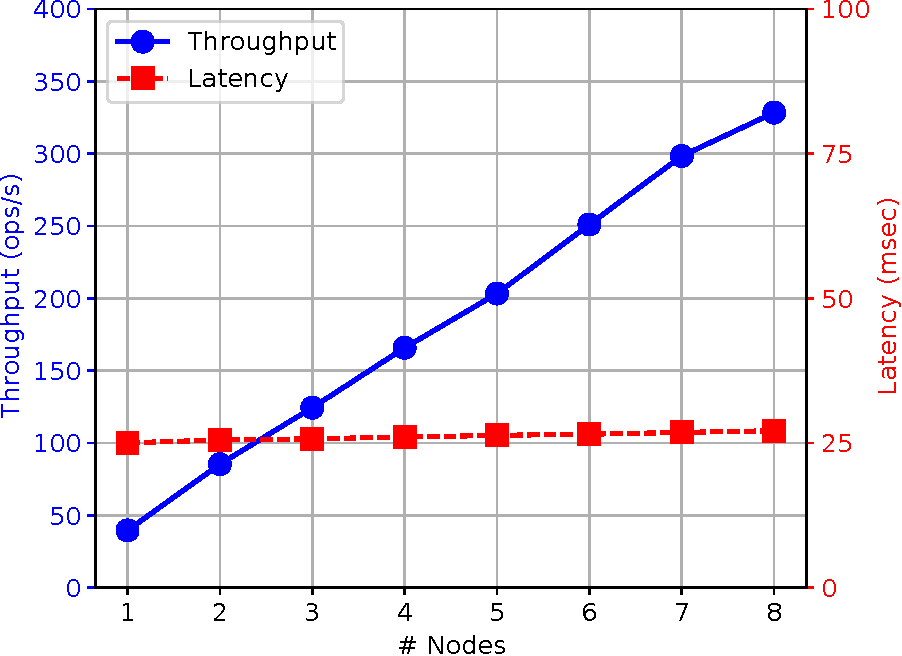
\includegraphics[width=\textwidth]{Graphs/scalability.pdf}
		\caption{Scalability: Overall throughput of the cluster and latency of each
			operation.}
		\label{grf:scalability}
	\end{subfigure}
	\par\bigskip
	\begin{subfigure}{0.45\textwidth}
		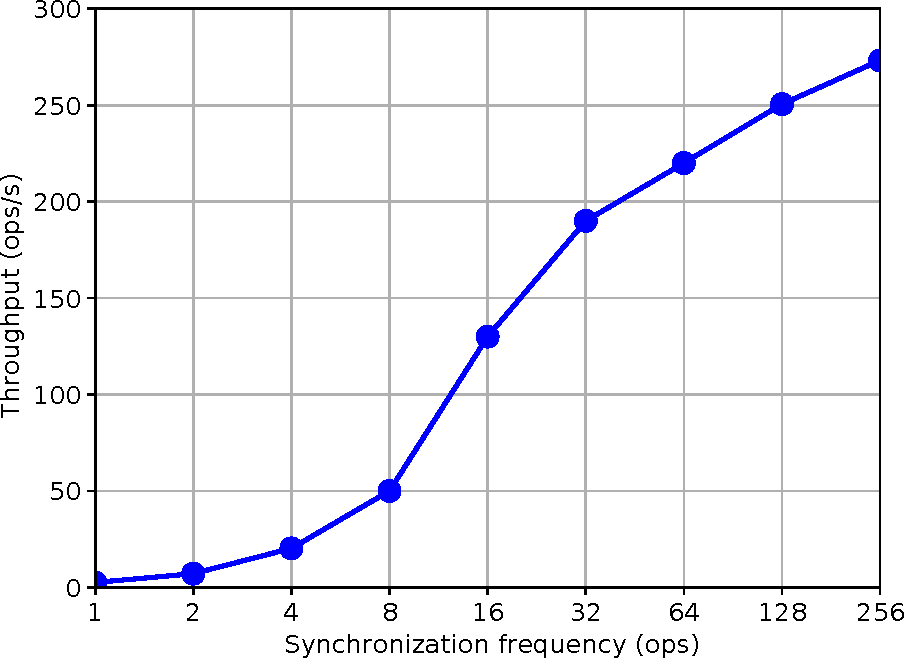
\includegraphics[width=\textwidth]{Graphs/synchronization.pdf}
		\caption{Synchronization: Overall throughput of the cluster while actively
			synchronizing with the successor node.}
		\label{grf:synchronization}
	\end{subfigure}
	\hfill
	\begin{subfigure}{0.45\textwidth}
		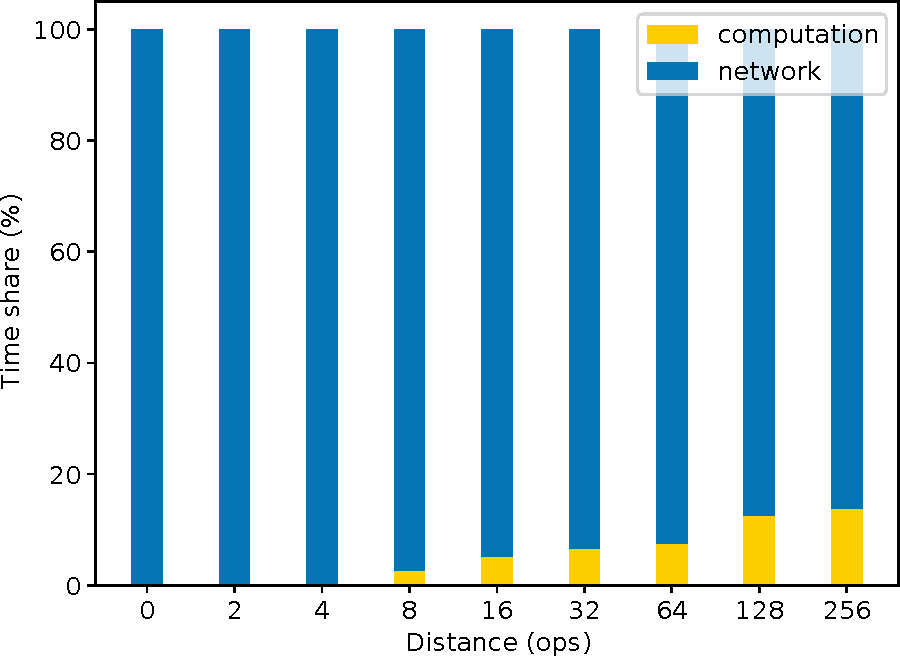
\includegraphics[width=\textwidth]{Graphs/merge.pdf}
		\caption{Merge performance: Cost of merging concurrent operations across
		nodes.}
		\label{grf:merge}
	\end{subfigure}
	\caption{\name performance evaluation.}
  \label{grf:evaluation}
\end{figure}

For our experiments, we instantiate an 8-node geo-distributed cluster in Google
Cloud Platform~\cite{gcp}. Each node is an \C{n1-standard-4} instance with 2
virtual CPUs and 7.5 GB of memory. The nodes are arranged in a ring as shown in
Figure~\ref{fig:cluster} and synchronize (push and pull updates) when necessary
with its successor. While \name does not impose any restrictions on
synchronizing with other nodes, we choose to only synchronize with the
successor since we are guaranteed eventual convergence with a ring cluster. If
the successor becomes unavailable, the node synchronizes with other available
nodes. Operations are generated and applied locally on each node before they
are propagated eventually to other nodes with the help of a background thread
that synchronizes with its successor every second.

\subsection{Results}

We evaluate the scalability of concurrent editing application by increasing the
cluster size from 1 to 8 (the 4 node ring cluster consists of nodes numbered 0
to 3), with each node performing concurrent edits to the same document. In each
case, we measure the overall cluster throughput and latency of each operation.
The results are presented in Figure~\ref{grf:scalability}. The results show
that the cluster throughput increases linearly with the number of concurrent
editors, while the latency for each operation remains the same. This is because
each operation is performed locally and does not require synchronization with
other nodes. The nodes remain available to accept requests even if the node
gets disconnected. Since the document type is mergeable, eventually when the
node comes back online, the updates are synchronized with the cluster.

While updates are propagated asynchronously, we also measured the impact of
propagating updates synchronously by forcing synchronization every few
operations. This corresponds to a partially synchronous system, which is also
unavailable; if the cluster is unreachable, local operations will not be
accepted. While this is not a realistic deployment, the results help us
understand the overhead of synchronization. The results are shown in
Figure~\ref{grf:synchronization}. The result show that frequent blocking
synchronization is prohibitively expensive with the throughput dropping to 3
ops/s for synchronizing after every operation. \name uses Git transfer protocol
for synchronization which involves multiple roundtrips between the nodes for
synchronization. But as the synchronizations get less frequent, we can see that
the throughput asymptotically approaches the asynchronous case
(Figure~\ref{grf:scalability}).

Finally, we evaluate the performance of merge functions. For this experiment,
we consider the nodes 1 (\C{us-central1-b}) and 2 (\C{europe-west1-b}). Both
nodes start with the initial document and perform \C{n} concurrent edits
without synchronization. After this, the nodes synchronize pushing the local
edits and pulling the remote edits, and merge to produce the final document. In
this case, we indicate the distance of synchronization as \C{2n}.
Figure~\ref{grf:merge} presents the time share between network and computation
for performing 3-way merge. We see that the merge time is dominated by the
network overhead. This is because of the transfer protocol involving multiple
roundtrips and the need to transfer objects not only for application objects
but also Git internal objects for history, directory structure and branches. We
observe that we can improve the network performance by implementing a streaming
protocol that eagerly transfers objects.

More importantly, the cost of computation grows sub-linearly. This is because
of efficient merge function on ropes enabled by Irmin's content-addressed
storage backend, and more expensive operational transformation of merging
concurrent edits to leaf nodes is invoked rarely on small strings.


\section{Related Work}
\label{sec:related}

Our idea of versioning state bears resemblance to Concurrent
Revisions~\cite{BBL+10}, a programming abstraction that provides
deterministic concurrent execution by forking and merging
\emph{versions}, portions of state shared among concurrent threads.
The idea of using revisions as a means to programming eventually
consistent distributed systems was further developed
in~\cite{BFL+12,Burckhardt2012}.  The \name\ programming model,
however, differs substantially from a concurrent revisions model
because it imposes no distinction between \emph{servers}, machines
that hold global state, and \emph{clients}, devices that operate on
local, potentially stale, data - any computation executing in a
distributed environment is free to fork new versions, and synchronize
against other replicated state.  Our model, furthermore, supports
fully decentralized operation and is robust to network partitions and
failures. Just as significantly, \name\ allows applications to
customize join semantics with programmable merge operations.  Indeed,
the integration of a version-based mechanism within OCaml allows a
degree of type safety, composability, and profitable use of
polymorphism not available in related systems.

\cite{Burckhardt2015} also presents an operational model of a
replicated data store that is based on the abstract system model
presented in ~\cite{Burckhardt2014}; their design is similar to the
model described in~\cite{pldi15}.  In both approaches, coordination
among replicas involves transmitting operations on replicated objects
that are performed locally on each replica.  In contrast,
\name\ allows programmers to use familiar state-based and functional
abstractions when developing distributed applications.  As we
illustrated in Fig.~\ref{fig:counter-rdt}, using effects and
operations to coordinate the activities of replicas may involve
addressing subtleties that do not manifest otherwise.  Our case
studies and experimental results support our contention that using
well-understood state (heap)-based abstractions to build distributed
applications greatly simplifies program reasoning and eases
development, without compromising efficiency.

Modern distributed systems are often equipped with only parsimonious
data models (e.g., key-value model) and poorly understood low-level
consistency guarantees\footnote{Cassandra~\cite{Cassandra}, a popular
  NoSQL data store, comes with various consistency enforcement
  mechanisms, such as anti-entropy protocols, {\sc QUORUM} and {\sc
    LOCAL\_QUORUM} reads and writes, and light-weight transactions,
  each of which can be controlled via configuration knobs or runtime
  parameters.}  that complicate program reasoning, and make it hard to
enforce application integrity. Some authors~\cite{bailis-bolton} have
demonstrated that it is possible to\emph{bolt on} high-level
consistency guarantees (e.g., causal consistency)~\cite{COPS,BEG+17}
as a \emph{shim layer} service over existing stores.

A number of verification techniques, programming abstractions, and
tools have been proposed to reason about program behavior in a
geo-replicated weakly consistent environment.  These techniques treat
replicated storage as a black box with a fixed pre-defined consistency
model~\cite{bailis-vldb, alvaro-calm, gotsman-popl16,redblue-atc,
  redblue-osdi, ecinec}.  On the other hand, compositional proof
techniques and mechanized verification frameworks have been developed
to rigorously reason about various components of a distributed data
store~\cite{verdi,lbc16}. \name seeks to provide a rich high-level
programming model, built on rigorous foundations, that can facilitate
program reasoning and verification.  An important by-product of the
programming model is that it does not require algorithmic
restructuring to transplant a sequential or concurrent program to a
distributed, replicated setting; the only additional burden imposed on
the developer is the need to provide a merge operator, a function that
can be often easily written for many common datatypes.

Several conditions have been proposed to judge whether an operation on
a replicated data object needs coordination or not. ~\cite{Calm}
defines \emph{logical monotonicity} as a sufficient condition for
coordination freedom, and proposes a consistency analysis that marks
code regions performing non-monotonic reasoning (eg: aggregations,
such as \C{COUNT}) as potential coordination
points. ~\cite{IConfluence} and ~\cite{Sieve} define \emph{invariant
  confluence} and \emph{invariant safety}, respectively, as conditions
for safely executing an operation without coordination.
~\cite{indigo} requires programmers to declare application semantics,
and the desired application-specific invariants as formulas in
first-order logic. It performs static analysis on these formulas to
determine $I$-offender sets - sets of operations, which, when
performed concurrently, result in violation of one or more of the
stated invariants. For each offending set of operations, if the
programmer chooses invariant-violation avoidance over violation
repair, the system employs various techniques, such as escrow
reservation, to ensure that the offending set is effectively
serialized.  All of these approaches differ significantly from the
core goals of \name, which is to enable seamless application-driven
techniques for programming geo-replicated systems.  The
\name\ programmer is not concerned with different system-specific
consistency or isolation levels, or invariants that are sensitive to
these levels.  Instead, the only requirements demanded of the
developer is the need to reason about a sensible merge semantics for
data structures.  Such reasoning can be applied without consideration
of system- or architecture-specific details.  This reasoning phase
implicitly expresses salient semantic invariants without having to be
exposed to low-level operational details.

There have been numerous proposals over the years for realizing
distributed functionality in a functional programming context.
Poly/ML~\cite{Mat97} and Facile~\cite{TLK+93} both extend Standard ML
with distributed programming abstractions.  Kali-Scheme~\cite{CJK95}
defines a distributed extension for Scheme-48, and Cloud
Haskell~\cite{EBPJ11} describes a domain-specific language that
enables development of distributed Haskell programs.
Obliq~\cite{Car95} explores issues related to mobility, lexical
scoping, and network references in an object-oriented framework that
enables safe (i.e., lexical) transmission of closures.  However,
unlike \name, none of these systems consider issues of object
replication or consistency as central to their programming models.
The realities of modern-day scalable distributed systems, especially
those that are constructed from geographically distributed
participants, dictate that we must necessarily grapple with
consistency issues to achieve any kind of reasonable performance; it
is noteworthy that replication is inherent in many widely-used
distributed system implementations today (e.g.,
Cassandra~\cite{Cassandra} or Dynamo~\cite{Dynamo}), which provide
only weak consistency guarantees.  Rather than providing, as other
approaches have, a low-level operational treatment of replication, our
primary contribution is the development of a principled high-level
approach to framing issues of consistency and replication.  Our goal
is to leverage functional programming principles to minimize
disruption to the way programmers structure and reason about their
applications, without compromising efficiency or performance.  Indeed,
the semantics of mergeable types and versioning has utility in any
concurrent setting that must deal with non-trivial coordination and
synchronization costs, even without taking distribution or replication
issues into account.


\section{Conclusions}
\label{sec:conclusions}

Replication is a critical feature in geo-distributed systems used to
improve latency and availability.  Existing approaches to dealing with
replicated data often involve complex and subtle code restructuring,
and the use of specialized datatypes that interact poorly with other
language structures.  \name\ is a programming model that extends ML
with implicit support for replication that overcomes these concerns.
Its notion of concurrency and synchronization is encapsulated within a
monad that considers distrbuted computation in terms of typed versions
of replicated state.  Notably, any ML data structure can participate
in a distributed computation using this monad by providing a merge
function that dictates how different versions of that structure can be
reconciled.  Our versioning semantics enjoys strong consistency and
progress guarantees that make it useful in a fully decentralized (and
unreliable) cloud environment.  Furthermore, our experimental results
demonstrate that using such high-level abstractions need not come at
the expense of efficient implementations.


%% Acknowledgments
% \begin{acks}                            %% acks environment is optional
%                                         %% contents suppressed with 'anonymous'
%   %% Commands \grantsponsor{<sponsorID>}{<name>}{<url>} and
%   %% \grantnum[<url>]{<sponsorID>}{<number>} should be used to
%   %% acknowledge financial support and will be used by metadata
%   %% extraction tools.
%   This material is based upon work supported by the
%   \grantsponsor{GS100000001}{National Science
%     Foundation}{http://dx.doi.org/10.13039/100000001} under Grant
%   No.~\grantnum{GS100000001}{nnnnnnn} and Grant
%   No.~\grantnum{GS100000001}{mmmmmmm}.  Any opinions, findings, and
%   conclusions or recommendations expressed in this material are those
%   of the author and do not necessarily reflect the views of the
%   National Science Foundation.
% \end{acks}


%% Bibliography
\bibliography{all}


%% Appendix
%\appendix
%\section{Appendix}
\begin{figure}

\begin{subfigure}[b]{0.7\textwidth}
\begin{ocaml}
module type MList = sig
  module A: MERGEABLE
  include MERGEABLE
  type t = A.t list [@@deriving versioned]
  type edit = I of A.t * int
    | D of int
    | S of int * A.t * A.t
    | Nop
  ... (* All the standard list functions *)
  val insert: A.t -> int -> t -> t
  val delete: int -> t -> t
  val subst: int -> A.t -> t
  val edit_seq: t -> t -> edit list option
  val op_transform: edit list -> edit list -> edit list
  val merge: t -> t -> t -> t
end
\end{ocaml}
\caption{Signature of Mergeable Lists}
\label{fig:mlist-sig}
\end{subfigure}

\begin{subfigure}{0.75\textwidth}
\begin{ocaml}
(*
 * We reduce the problem of transforming op1* w.r.t op2* 
 * first to the problem of transforming op1* w.r.t op2,
 * and then to the problem of transforming op1 w.r.t op2.
*)
let op_transform mine others = 
  (*
   * Transforms my edit w.r.t other edit, and also returns how 
   * edits following my edit will witness the other edit.
   *)
  let xform my other = 
    let f my' = (my',other) in
    let g other' = (my,other') in
      match (my,other)  with 
      | (I (x,j), I (_,i)) when (j>=i) -> f @@ I (x,j+1)
      | (D j, I (_,i)) when (j>=i) -> f @@ D (j+1)
      | (S (j,x,y), I (_,i)) when (j>=i) -> f @@ S (j+1,x,y)
      | (I (x,j), D i) when (j=i) ->  g @@ Nop
      | (I (x,j), D i) when (j>i) ->  f @@ I (x,j-1)
      | (D j, D i) when (j=i) -> (Nop, Nop)
      | (D j, D i) when (j>i) ->  f @@ D (j-1)
      | (S (j,x,y), D i) when (j=i) -> f @@ Nop
      | (S (j,x,y), D i) when (j>i) -> f @@ S (j-1,x,y)
      | (I (x,j), S (i,y,z)) when (j<=i) -> g @@ S (i+1,y,z)
      | (D j, S (i,y,z)) when (j=i) -> g @@ Nop
      | (D j, S (i,y,z)) when (j<i) -> g @@ S (i-1,y,z)
      | (S (j,x,y), S (i,_,z)) when (j=i) -> f @@ S (j,x,A.merge x y z) 
      | _ -> f @@ my in
  let mine' = 
    List.fold_left 
      (fun mine other -> 
         let (mine',_) = 
           List.fold_left 
             (fun (xformed, other) my -> 
                let (my',other') = xform my other in
                  (xformed@[my'],other')) 
             ([],other) mine in
           mine') 
      mine others in
    mine'
\end{ocaml}
\caption{Operational transformation of list operations}
\label{fig:mlist-xform}
\end{subfigure}

\caption{Mergeable List Implementation}
\label{fig:mlist}
\end{figure}

\begin{lemma} [\bfseries Unique External Locus]
Every version $v$ (except the \C{INIT} version) in the history $H$
generated by the rules in Fig.~\ref{fig:opsem} has a unique external
locus.
\end{lemma}
\begin{proof}
By case analysis on the reduction relation. In each case, we assume
that the unique external locus property holds for the initial history,
and prove that it holds for the final history.

In \rulelabel{E-Run} case, initial version is the unique external locus of
the new version on the new branch $H(t)$. In \rulelabel{E-Fork} case,
which creates the branch $H(t')$ by forking from $H(t)$, the latest
version on $H(t)$ is the external locus of the first version on
$H(t)$. In \rulelabel{E-Push} case, the version on $H(t)$ has the same
external locus as the previous latest version, which, premise says, is
unique. No new version is created in \rulelabel{E-Pull}. In
\rulelabel{E-Pull-Wait}, new version is created by merging the latest
version ($v'$) on $H(t')$ into the latest version $v$ on $H(t)$.
Premise says that $v$ has a unique external locus (call it $v_o$). The
new version $v_m$ inherits $v_o$ as a least external ancestor, and
also has $v'$ as another least external ancestor. However, since
$\under{H}{v' \mbleto v}$, we have $\under{H}{v_o \preceq v'}$, we
have $v'$ as the the external locus.
\qed
\end{proof}

\begin{lemma} [\bfseries Unique LCA]
Every pair of versions $v_1$ and $v_2$ in the history $H$ generated by
the rules in Fig.~\ref{fig:opsem} have a unique least
common ancestor. 
\end{lemma}
\begin{proof}
By case analysis on the step relation. In each case, we assume that
the unique LCA property holds for the initial history, and prove that
it holds for the final history.

The \rulelabel{E-Run} case is trivial. The \rulelabel{E-Push} case
creates a new version ($v$) with \C{PUSH} tag at the end of a branch.
Let $v_1$ be the previous version on the branch, and let $v_2$ be any
other version. The premise is that $v_1$ and $v_2$ have a unique LCA
$v_0$. Observe that $v$'s internal locus is $v_1$ and its external
locus is same as that of $v_1$. Hence, all ancestors of $v_1$
(including itself) are also ancestors of $v$. Moreover, $v$ has no new
ancestors except itself, which is the latest version being added.
Hence, any common ancestor of $v_1$ and $v_2$ is also a common
ancestor of $v$ and $v_2$, while there cannot be new common ancestors.
Hence LCA of $v$ and $v_2$ is unique. The reasoning for
\rulelabel{E-Fork} is similar. The \rulelabel{E-Pull} case is trivial. 

The \rulelabel{E-Pull-Wait} case is where the merge happens. Version
$v'$ is merging into version $v$ to produce the next version $v_m$.
Let $v_2$ be any version. From the premise, we know that $v$ and $v_2$
have a unique LCA (call it $v_0$), and $v'$ and $v_2$ have a unique
LCA (call it $v_1$). But, we know that $v_2$ has a unique external
locus (call it $v_3$), hence we know that 
\begin{itemize}
  \item Both $v_0$ and $v_1$ are external ancestors of $v_2$. Hence,
  $\under{H}{v_0 \preceq v_3} \conj \under{H}{v_1 \preceq v_3}$.
  Since $\under{H}{v_0 \preceq v_m} \conj \under{H}{v_1 \preceq v_m}$, 
  $v_2$ and $v_m$ have a unique LCA.

  \item $v_0$ is an internal ancestor of $v_2$, hence an external
  ancestor of $v$, hence an external ancestor of $v_m$. $v_1$ is
  an ancestor of $v'$, hence also an external ancestor of $v_m$. 
\end{itemize}
\end{proof}






\end{document}
